\documentclass{article}
\usepackage[UTF8]{ctex}
\usepackage{pythonhighlight}

% Language setting
% Replace `english' with e.g. `spanish' to change the document language
\usepackage[english]{babel}
\usepackage{float}
% Set page size and margins
% Replace `letterpaper' with `a4paper' for UK/EU standard size
\usepackage[letterpaper,top=2cm,bottom=2cm,left=3cm,right=3cm,marginparwidth=1.75cm]{geometry}

% Useful packages
\usepackage{amsmath}
\usepackage{graphicx}
\usepackage[colorlinks=true, allcolors=black]{hyperref}




\title{数字逻辑设计期末课程设计}
\author{雷远航 \ 祝广程}

\begin{document}

\setcounter{tocdepth}{5}  % 显示几级标题 这次需求只显示1级 写的是0



\maketitle

\begin{abstract}
数逻期末课程设计


\end{abstract}


\tableofcontents
\newpage



\section{小组成员}
雷远航   \ 学号:3210105807
祝广程   \ 学号:3210105954


\section{项目介绍}
该项目主要利用verilog HDL语言设计实现了一个简单的LC3汇编语言机器码指令控制器,即模拟实现了一个单周期CPU。该CPU可以在一个时钟周期内对输入的一条指令进行处理,通过ALU、ControlUnit等模块对内存、寄存器的内容进行读写。其处理的指令集主要包括三大类:运算指令,如ADD、SUB等算术运算指令和AND、OR等逻辑运算指令;传输指令,如读取内存指令LDR、写入内存指令STR、压入栈指令PUSH、弹出栈指令POP;流程控制指令,如条件跳转指令BR、无条件跳转指令JMP、终止指令HALT(详见Instruction Table)。每条指令对应固定的机器码,机器码长度为16位,同时CPU中存放在寄存器和内存中的数据的大小也均为16位。通过执行一系列指令后寄存器的值是否与预期相符,可以验证CPU设计的正确性。

具体的指令集将在附录中给出.


\section{开发模式}
由github进行协作开发,最终的commit记录在附录中给出.

\section{框架思路}

\subsection{基本流程}
CPU在处理指令时,一般需要经过以下几个步骤: 

(1) 取指令(IF):根据程序计数器PC中的指令地址,从存储器中取出一条指令,同时,PC根据指令的字节长度自动递增,按顺序指向下一条指令所在的地址,但如果执行的是“流程控制”指令,则该指令指定的地址会被传入到PC中,实现指令的跳转执行。 

(2) 指令译码(ID):对取指令操作中得到的指令进行分析并译码,确定这条指令需要完成的操作,从而产生相应的操作控制信号,用于驱动执行状态中的各种操作。 

(3) 指令执行(EXE):根据指令译码得到的操作控制信号,具体地执行指令动作,然后转移到结果写回状态。

(4) 存储器访问(MEM):所有需要访问存储器的操作都将在这个步骤中执行,该步骤给出存储器的数据地址,把数据写入到存储器中数据地址所指定的存储单元或者从存储器中得到数据地址单元中的数据。 

(5) 结果写回(WB):指令执行的结果或者访问存储器中得到的数据写回相应的目的寄存器中。

\subsection{数据通路}
根据指令执行的五个阶段,我们设计出了如下图所示的数据通路图

各模块的功能和具体实现细节将在下一节中给出,在这一节中,我们主要阐述各控制信号的作用和三大类指令的执行过程,从而说明设计的总体框架和思路。
\subsubsection{DataPath图}
\begin{figure}[H]
    \centering
    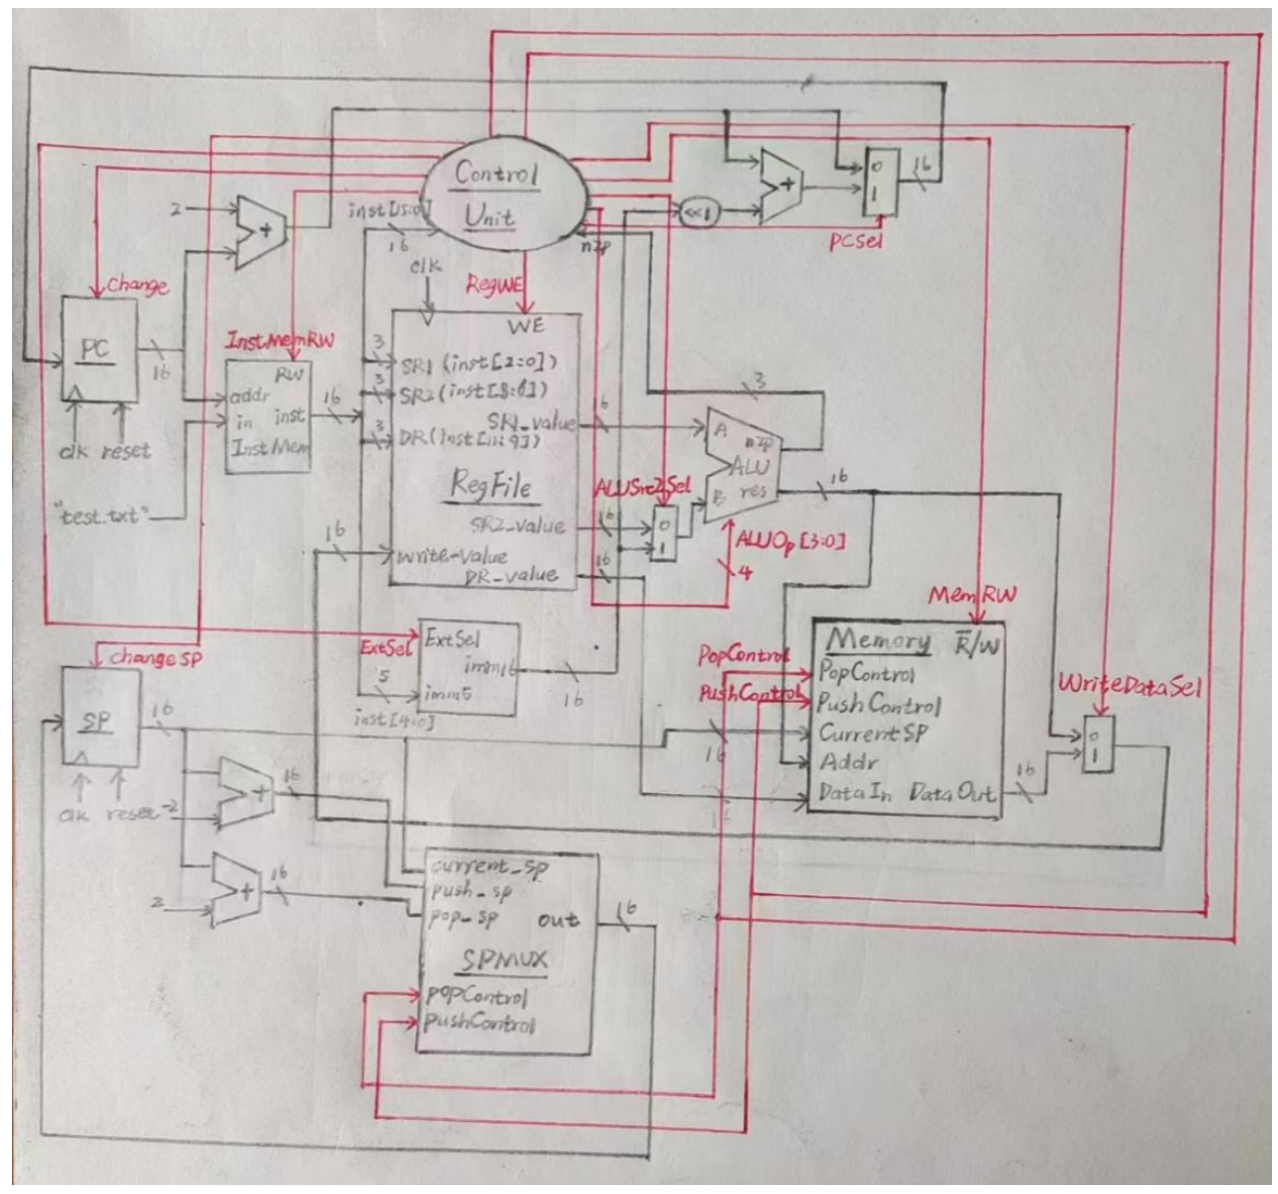
\includegraphics[width=0.7\textwidth]{pic/8.png}
    \end{figure}

\subsubsection{控制信号解释}
    \begin{figure}[H]
        \centering
        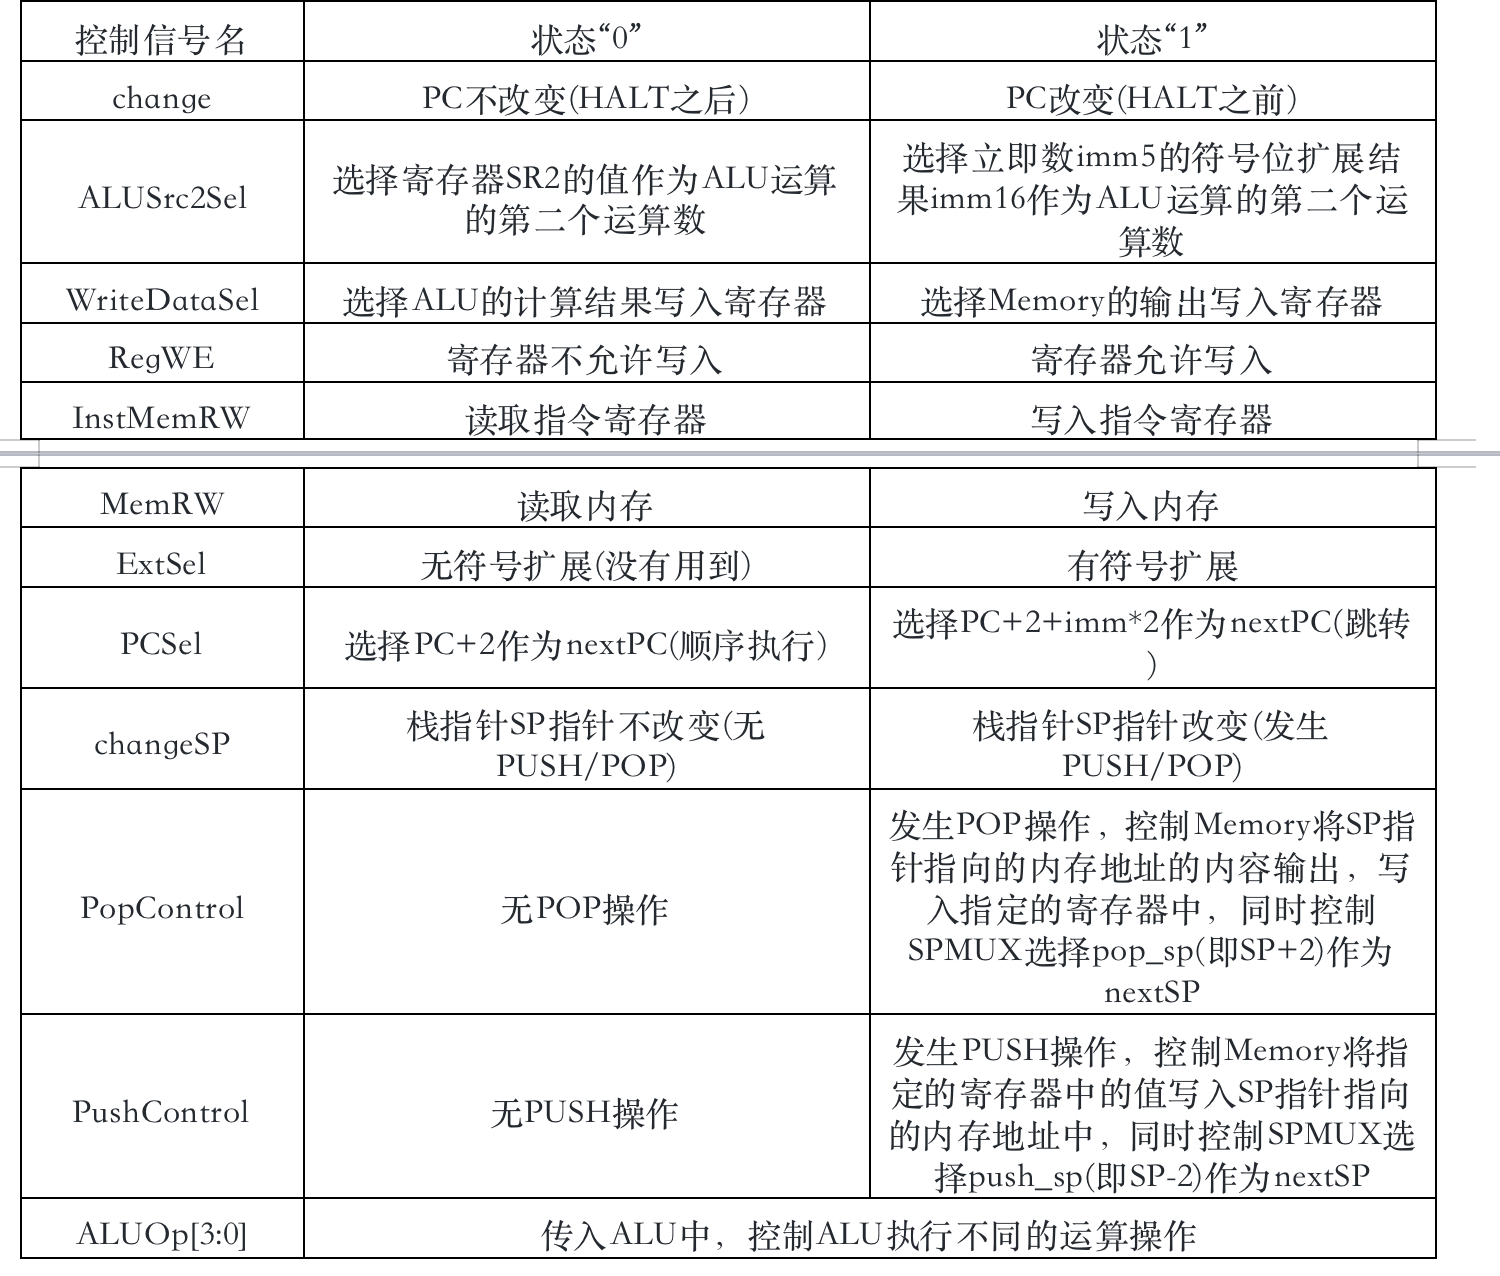
\includegraphics[width=0.7\textwidth]{pic/9.png}
        \end{figure}

\subsection{运行流程}
了解了各控制信号的作用之后,下面我们将根据IF、ID、EXE、MEM、WB五个阶段,分别以ADD、LDR、PUSH、BR、HALT五个指令为例阐述运算指令、传输指令和流程控制指令的运行机制,进而帮助读者理解该CPU设计的总体思路(建议对照数据通路图理解下面的流程)。

\subsubsection{IF阶段}
首先,在取指令(IF)阶段,PC的值会作为addr参数传入InstMem中,根据该地址输入,InstMem模块会读取并输出相应的16位指令(说明:InstMem模块会在initial阶段从外部文件,如“test.txt”中,读取要执行的所有指令并存放在一个数组当中)。同时,PC的值会加2,指向当前指令的下一条指令所在地址。至于为什么PC要加2,而不是1,是因为InstMem模块从外部文件中读取指令时,是以字节为单位读取的,并把读取的内容存放在一个每单元8位的数组当中,而我们的指令是16位的,因此从InstMem中获得指令,需要读取其数组中两个单元的内容,故PC指向的数组地址要加2。

\subsubsection{ID阶段}
然后,在指令译码(ID)阶段,InstMem模块会根据16位指令,提取相关有用的信息,如操作码(opcode)、目的寄存器(DR)、源寄存器(SR1/SR2)、立即数(imm5)等,并将其分别传输到Control Unit、Reg File、imm5Extend等模块中,Control Unit会发出相应的控制信号,辅助指令的执行。

\subsubsection{EXE阶段}
接着,在指令执行(EXE)阶段,imm5Extend模块会将立即数(imm5)扩展为16位,方便操作,RegFile模块会根据SR1、SR2、DR的值输出相应寄存器中的内容SR1\_value、SR2\_value、DR\_value,其中SR1\_value会作为ALU模块的A操作数,SR2\_value和imm16会根据ALUSrc2Sel信号,选择其一作为ALU模块的B操作数,ALU模块会对A、B两操作数进行运算,输出结果res,并根据res设置nzp的值(结果为负,则n为1;结果为零,则z为1;结果为正,则p为1)。

\subsubsection{MEM阶段}
此后,在存储器访问(MEM)阶段,res会作为Addr参数传入到Memory模块中,对于LDR/STR指令,Addr为SR1\_value+imm16的值,表示要操作的内存地址;而对于PUSH指令,Addr为SR1\_value的值,表示要写入内存堆栈的内容,这一点需要特别注意。PUSH/POP指令操作的堆栈的栈顶指针由currentSP给出,每次将数据压入或弹出堆栈时currentSP都会作出相应的移动(PUSH/POP指令如何工作详见下面对PUSH指令的分析)。另外,对POP、PUSH的识别通过PopControl与PushControl两个控制信号给出,读取的内存值会在DateOut输出。

\subsubsection{WB阶段}
最后,在结果写回(WB)阶段,会利用一个二选一多路选择器,根据WriteDataSel信号,从ALU的运算结果res和内存的读取值DataOut中选择其一,作为write\_value参数输入RegFile模块,当RegWE为1时,在时钟信号正边沿将数据写入目的寄存器DR当中。

\subsection{对指令执行的举例说明:}

\subsubsection{ALU指令}
ADD:取指令(IF)阶段和指令译码(ID)阶段参见上述分析,不做赘述。在指令执行(EXE)阶段,A操作数从RegFile的输出SR1\_value中得来,B操作数会根据ALUSrc2Sel信号选择SR2\_value和imm16其中一个,ALUSrc2Sel信号是由inst[5]决定的,当inst[5]等于0时,ALUSrc2Sel信号也为0,选择SR2\_value;当inst[5]等于1时,ALUSrc2Sel信号也为1,选择imm16。ALU计算完毕之后,没有存储器访问(MEM)的操作,直接进入结果写回(WB)阶段,WriteDataSel信号为0,选择ALU运算的结果res作为输出,RegWE为1,允许将res写入到目的寄存器DR当中。(其他的运算指令的执行过程均可参照ADD进行分析)

\subsubsection{内存存取指令}
LDR:取指令(IF)阶段和指令译码(ID)阶段参见上述分析,不做赘述。在指令执行(EXE)阶段,A操作数从RegFile的输出SR1\_value中得来,B操作数则选择imm16,将SR1\_value与imm16相加作为ALU运算的输出结果,即可得到要读取内存的地址。因此,在存储器访问(MEM)阶段,读取指定内存地址的内容并输出。在写回(WB)阶段,WriteDataSel信号为1,选择内存的读取值DataOut作为输出,RegWE为1,允许将DataOut写入到目的寄存器DR当中。(STR指令的执行过程可参照LDR进行分析)

\subsubsection{栈操作指令}
PUSH:取指令(IF)阶段和指令译码(ID)阶段参见上述分析,不做赘述。在指令执行(EXE)阶段,A操作数从RegFile的输出SR1\_value中得来,并直接将其作为ALU运算的结果res输出。在存储器访问(MEM)阶段,Addr即为要写入内存堆栈的内容,此时PushControl信号为1,控制Memory模块将Addr的值写入到currentSP指向的内存地址中,实现堆栈压入数据的操作。由于该操作不涉及寄存器的写入,故在写回(WB)阶段,RegWE为0,寄存器的内容保持不变。(POP指令的执行过程可参照PUSH进行分析)

对于PUSH和POP操作,还需要说明一下栈顶指针是如何移动的。栈顶指针currentSP存放在SP模块中,当changeSP信号为1时,currentSP就在时钟信号正边沿会根据输入的nextSP值发生改变。而nextSP则是由多路选择器SPMUX模块决定的,该模块包含三个数据输入current\_sp、pop\_sp和push\_sp,两个控制信号输入PushControl和PopControl,当发生PUSH操作时,PushControl为1,就选取push\_sp(current\_sp-2)作为nextSP,此时changeSP信号为1,故写入到SP模块当中,下一个时钟周期current\_sp就变为current\_sp-2;当发生POP操作时,PopControl为1,就选取pop\_sp(current\_sp+2)作为nextSP,此时changeSP信号为1,故写入到SP模块当中,下一个时钟周期current\_sp就变为current\_sp+2;而如果当前周期执行的指令既不是PUSH,也不是POP,就选取current\_sp作为nextSP,同时changeSP信号为0,下一个时钟周期current\_sp不会发生变化。

\subsubsection{流程控制指令}
BR:取指令(IF)阶段和指令译码(ID)阶段参见上述分析,不做赘述。在指令执行(EXE)阶段,BR指令会根据(inst[11]\&n | inst[10]\&z | inst[9]\&p)的值给出PCSel信号,当(inst[11]\&n | inst[10]\&z | inst[9]\&p)为1时,PCSel就为1,从而选择PC+2+2*imm16作为nextPC,如此在下一个时钟周期PC的值就会发生跳转;否则,PCSel为0,nextPC仍为PC+2,依旧顺序执行指令。(JMP指令的执行过程可参照BR进行分析)

\subsubsection{HALT}
HALT:该指令的工作机制很简单,就是当读到该指令时,change信号为0,PC就不再发生变化,从而终止程序。

\section{模块的具体实现}

\subsection{module PC}
\begin{figure}[H]
    \centering
    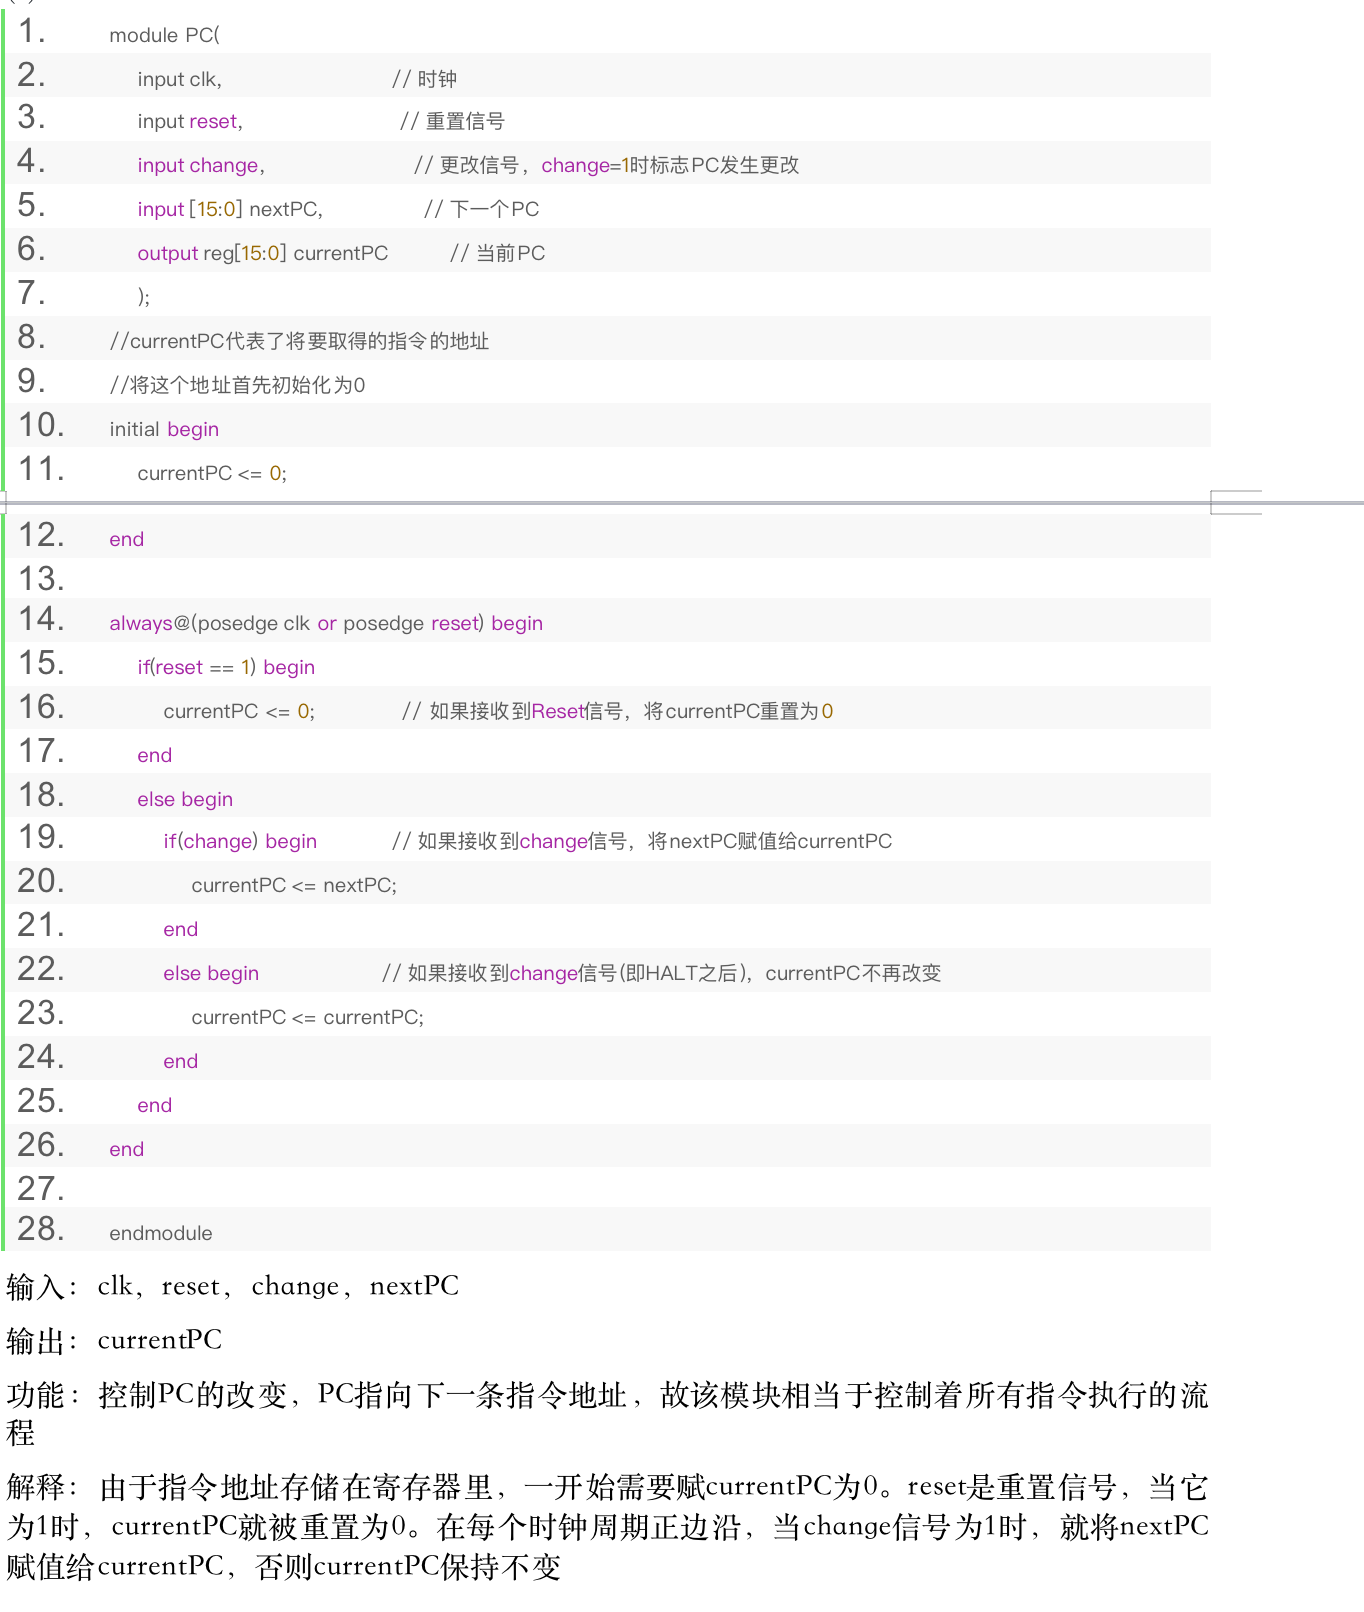
\includegraphics[width=0.8\textwidth]{pic/10.png}
   
    \end{figure}

\subsection{module InstMem}
\begin{figure}[H]
    \centering
    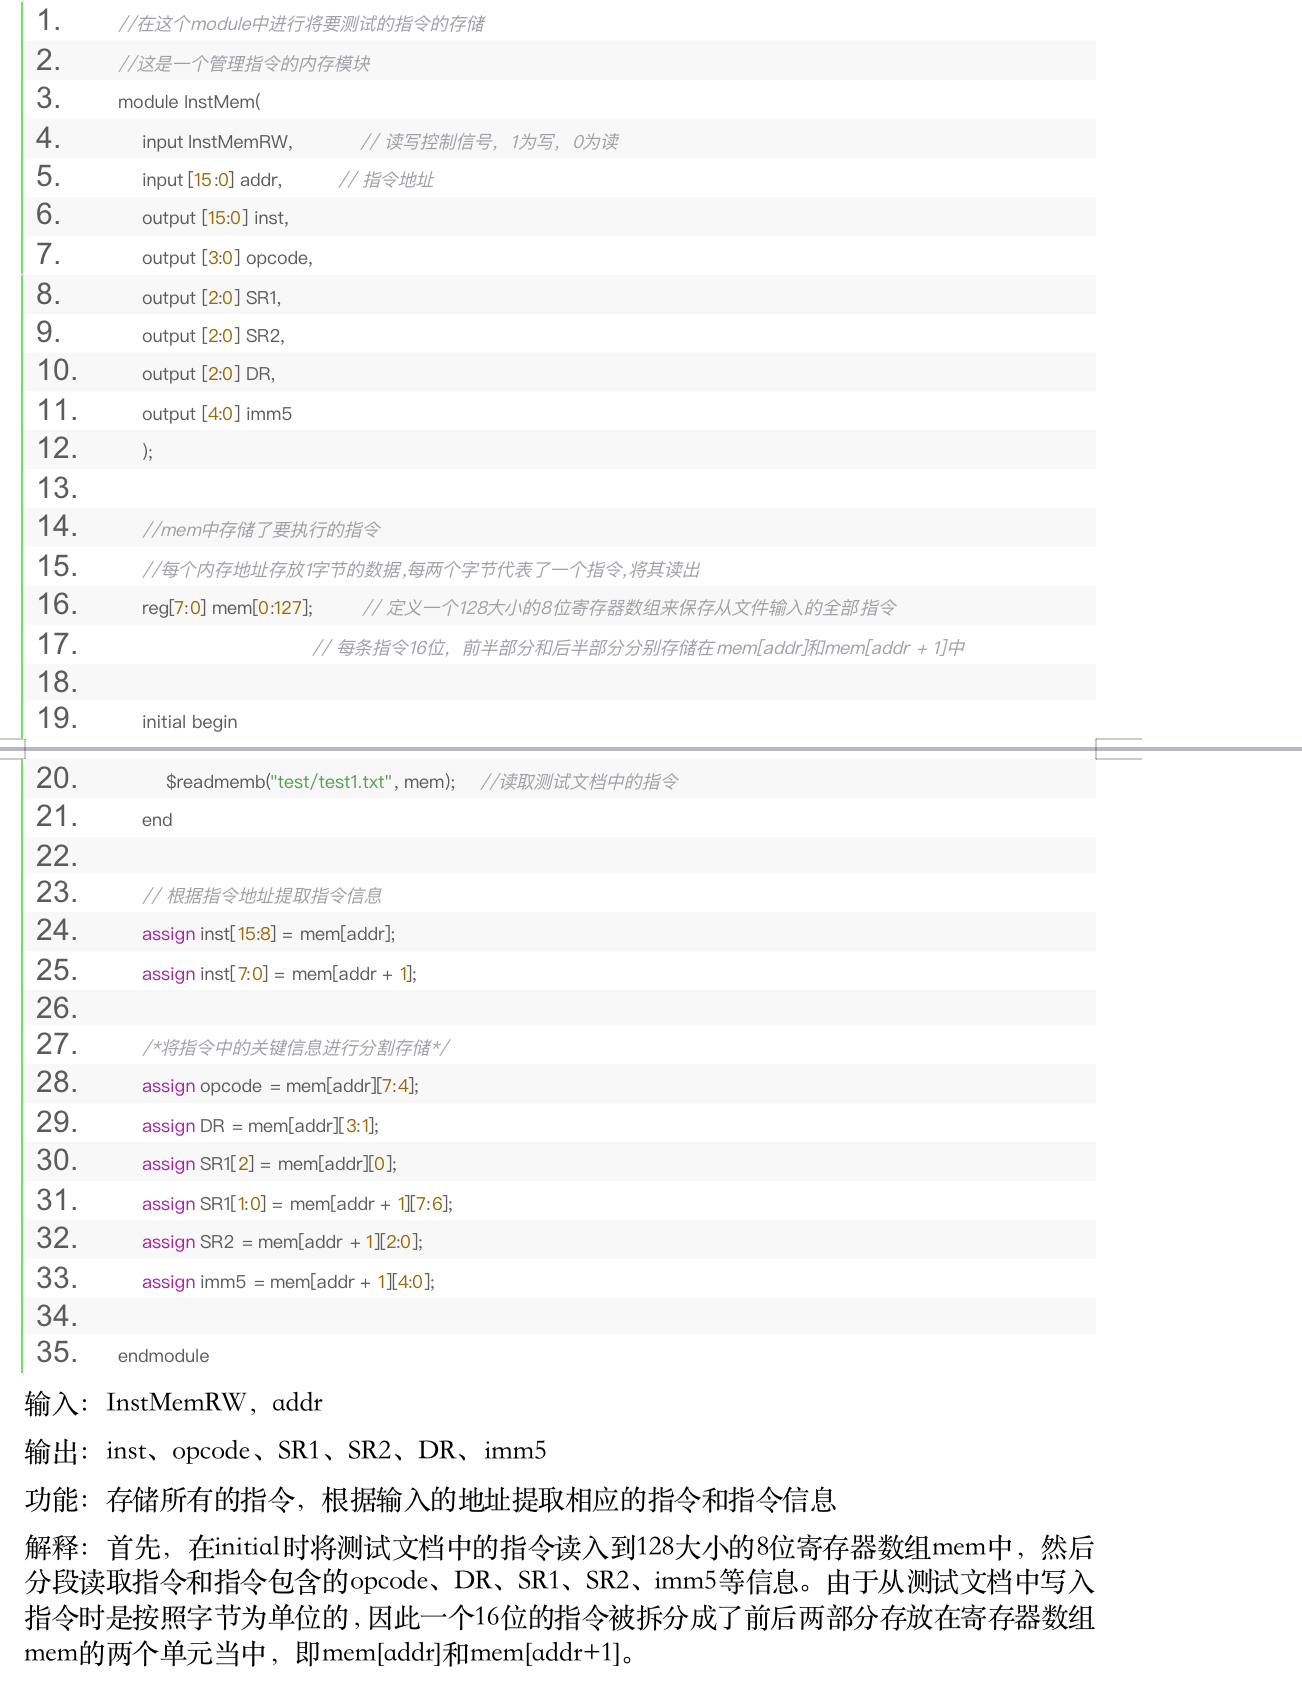
\includegraphics[width=1\textwidth]{pic/11.png}
  
    \end{figure}


\subsection{module RegFile}
\begin{figure}[H]
    \centering
    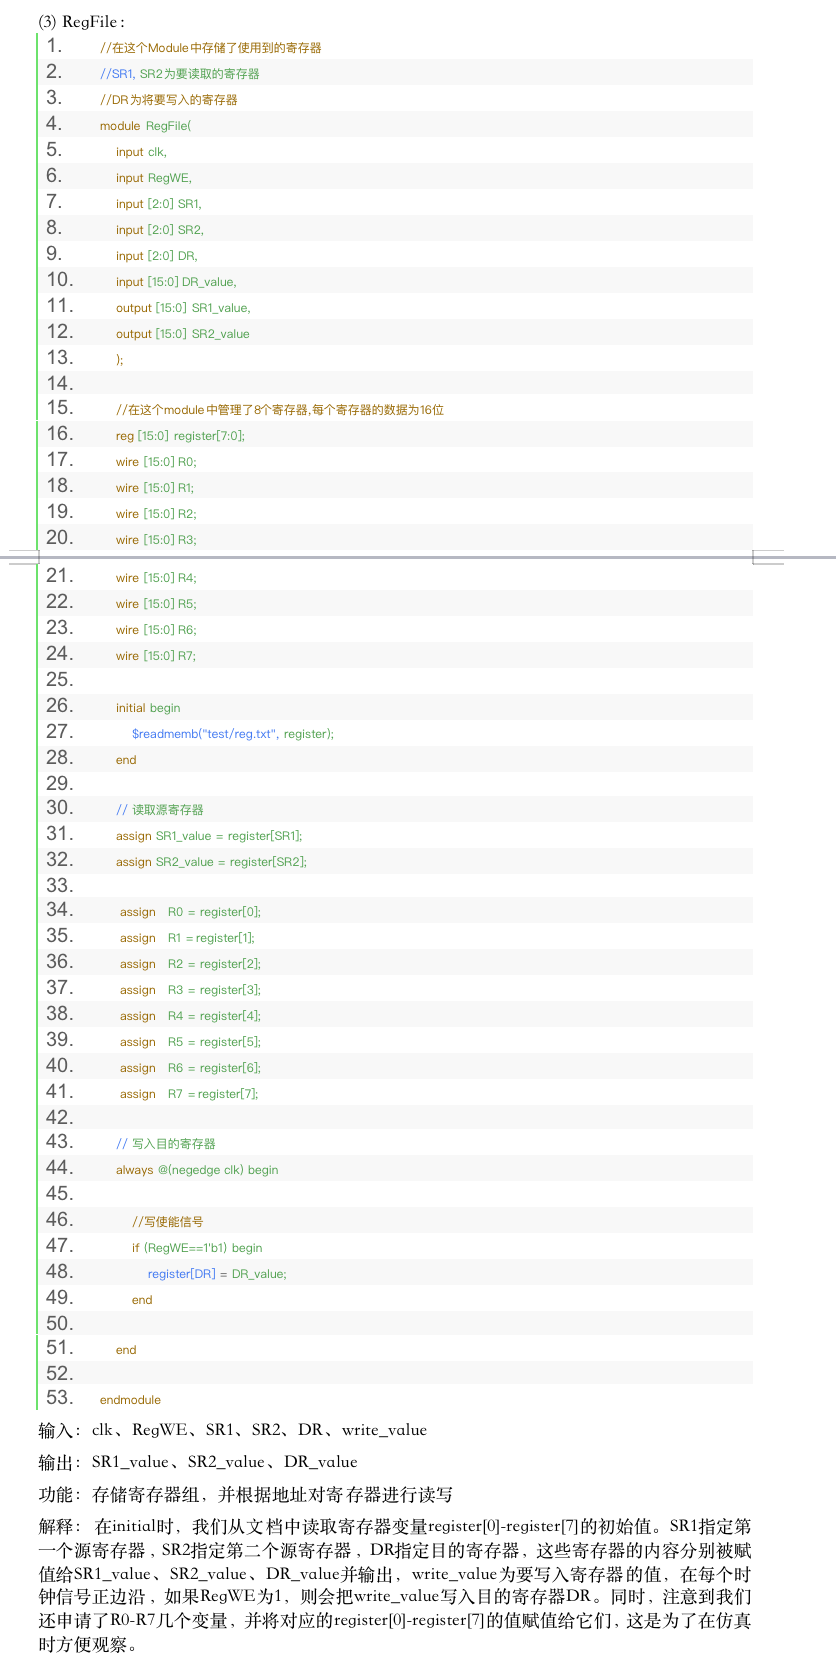
\includegraphics[width=0.7\textwidth]{pic/12.png}
  
    \end{figure}

\subsection{module ALU}
\begin{figure}[H]
    \centering
    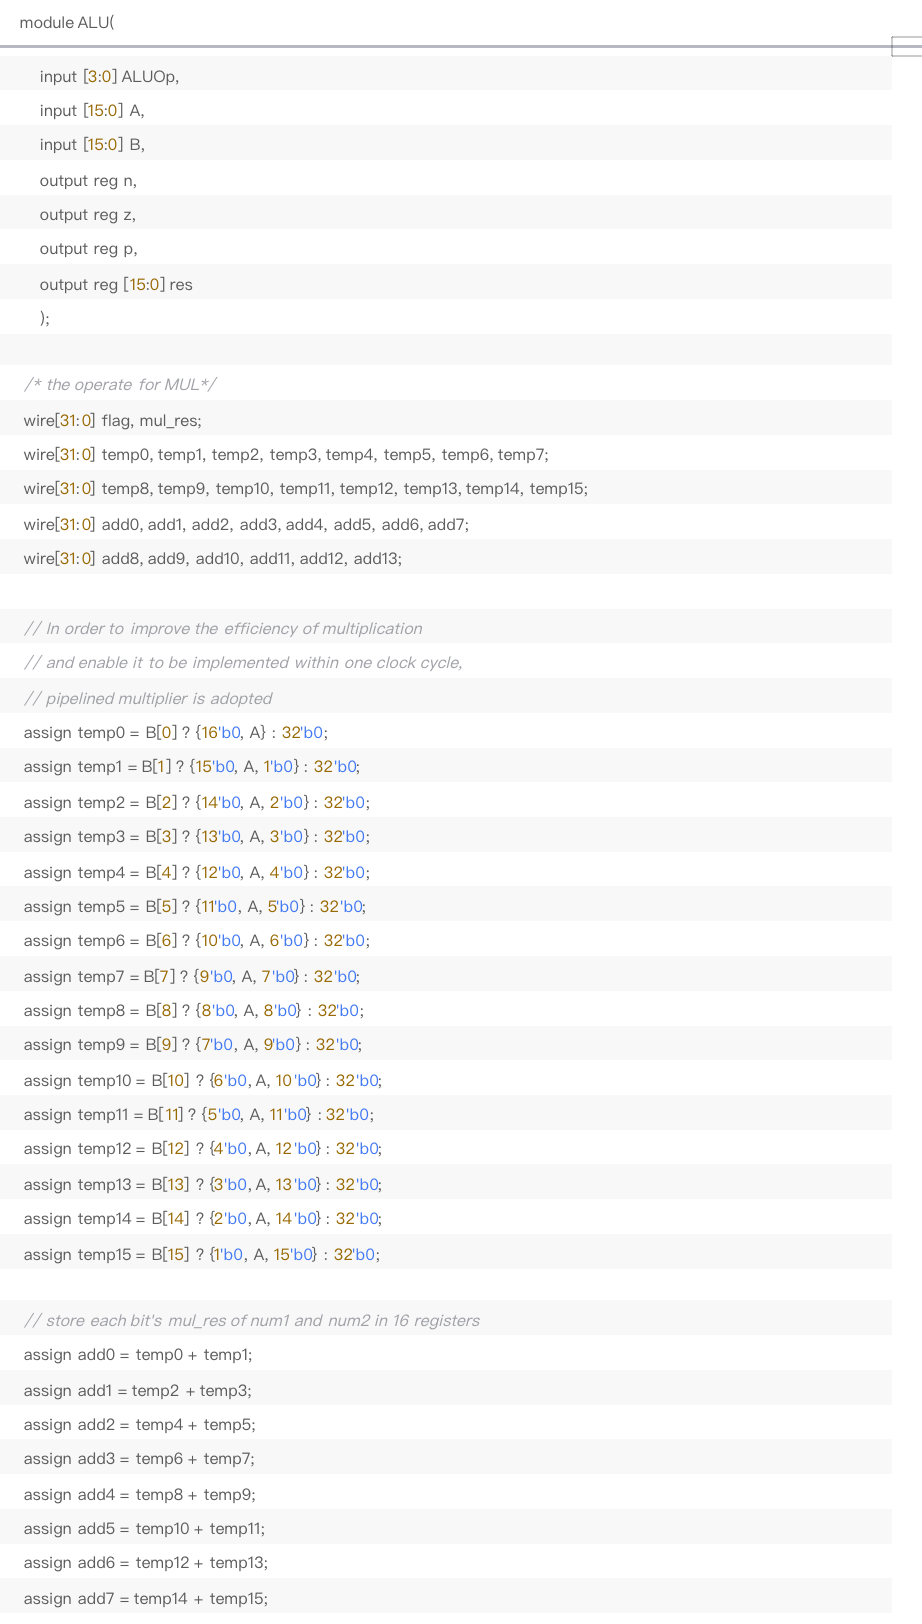
\includegraphics[width=0.8\textwidth]{pic/13.png}
  
    \end{figure}

    \begin{figure}[H]
        \centering
        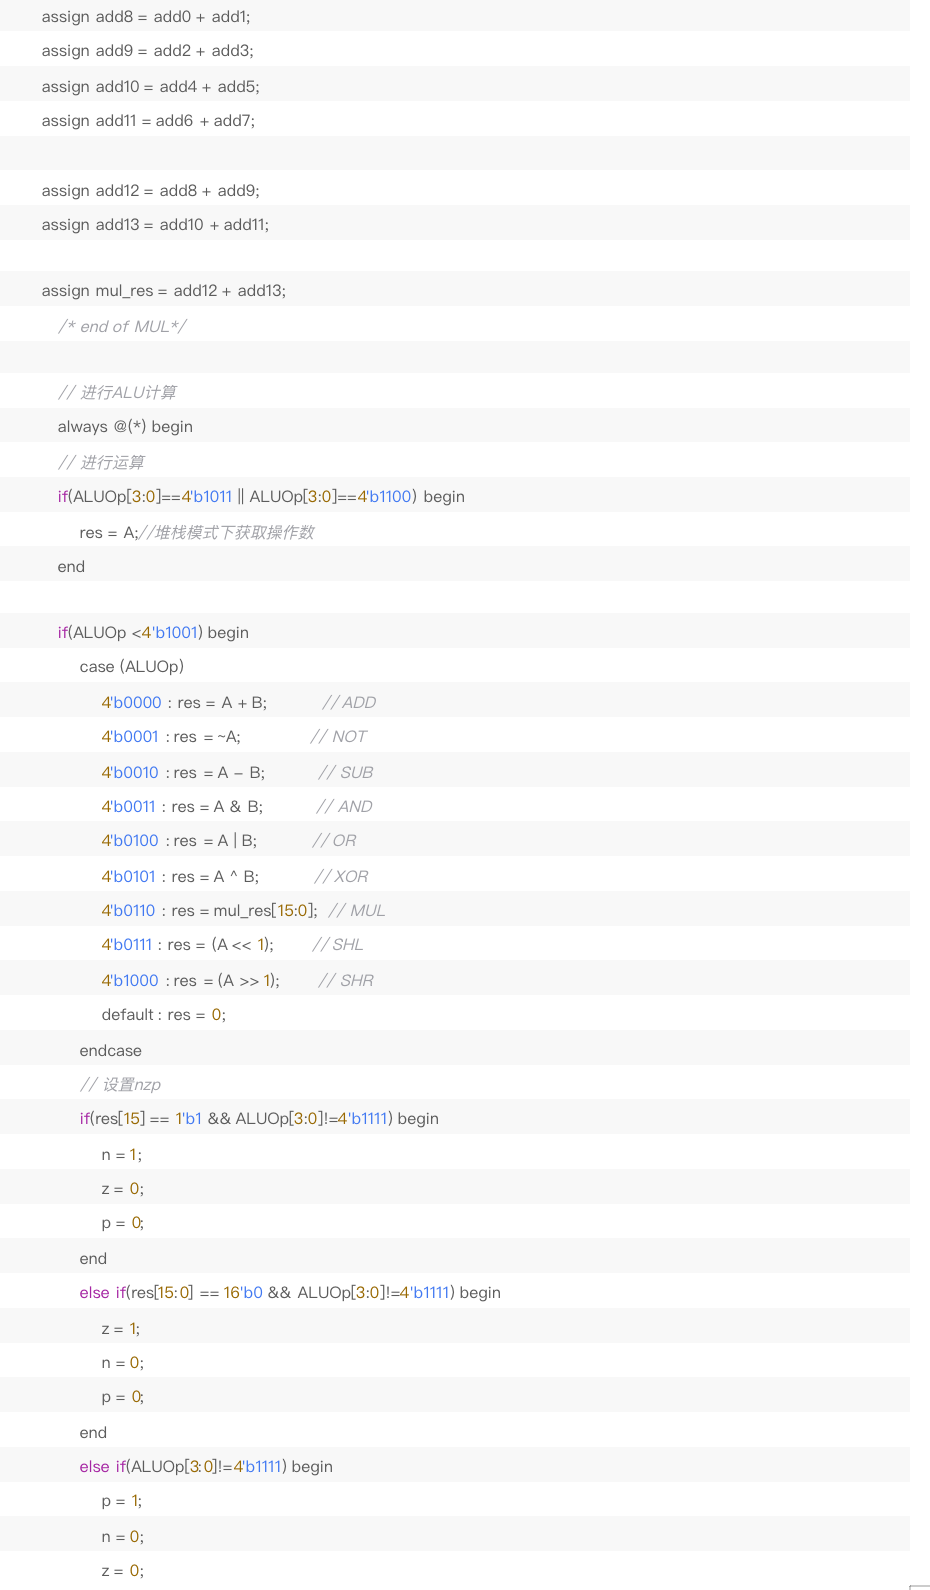
\includegraphics[width=0.8\textwidth]{pic/14.png}
      
        \end{figure}

        \begin{figure}[H]
            \centering
            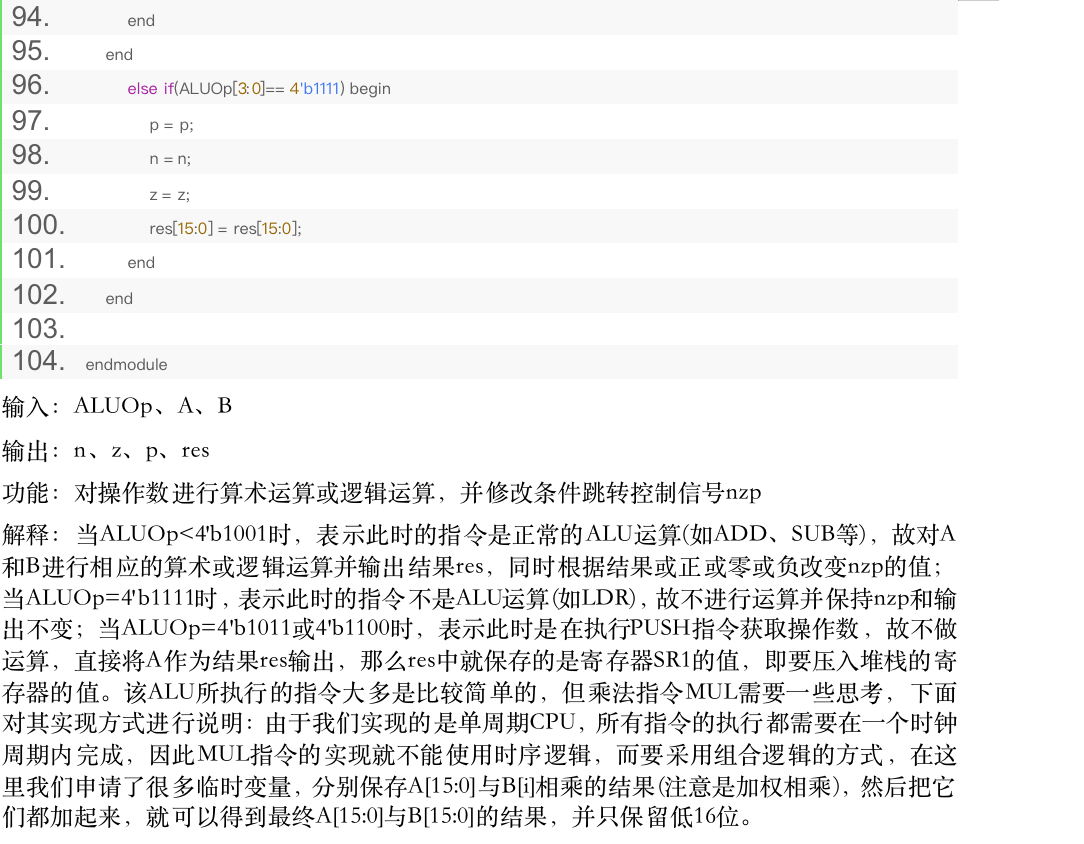
\includegraphics[width=0.8\textwidth]{pic/15.png}
          
            \end{figure}

\subsection{module Imm5Extend}
\begin{figure}[H]
    \centering
    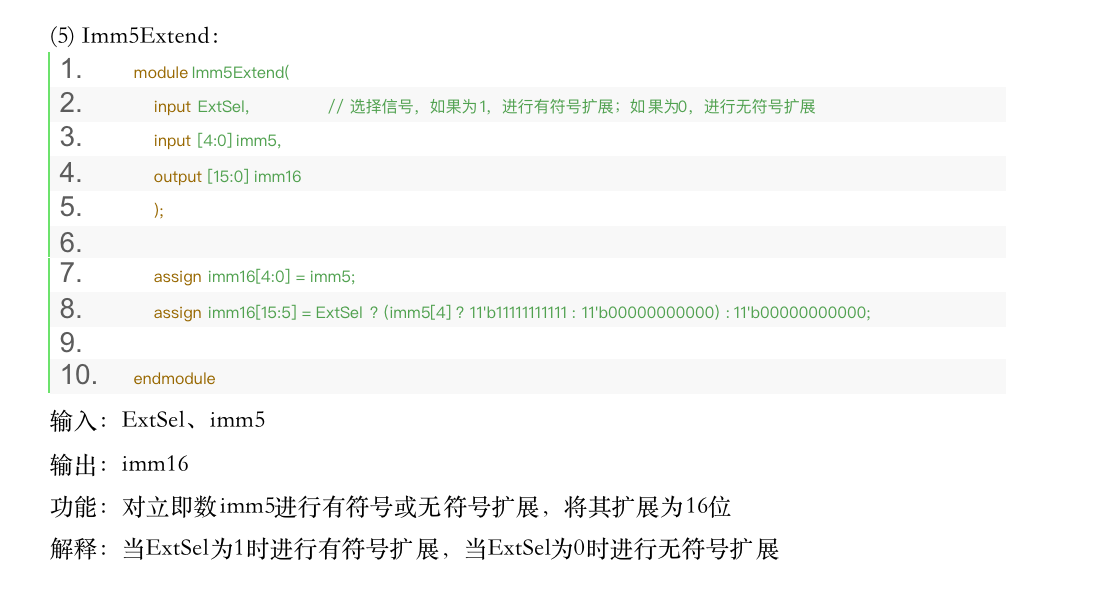
\includegraphics[width=0.8\textwidth]{pic/16.png}
  
    \end{figure}


\subsection{module Memory}
\begin{figure}[H]
    \centering
    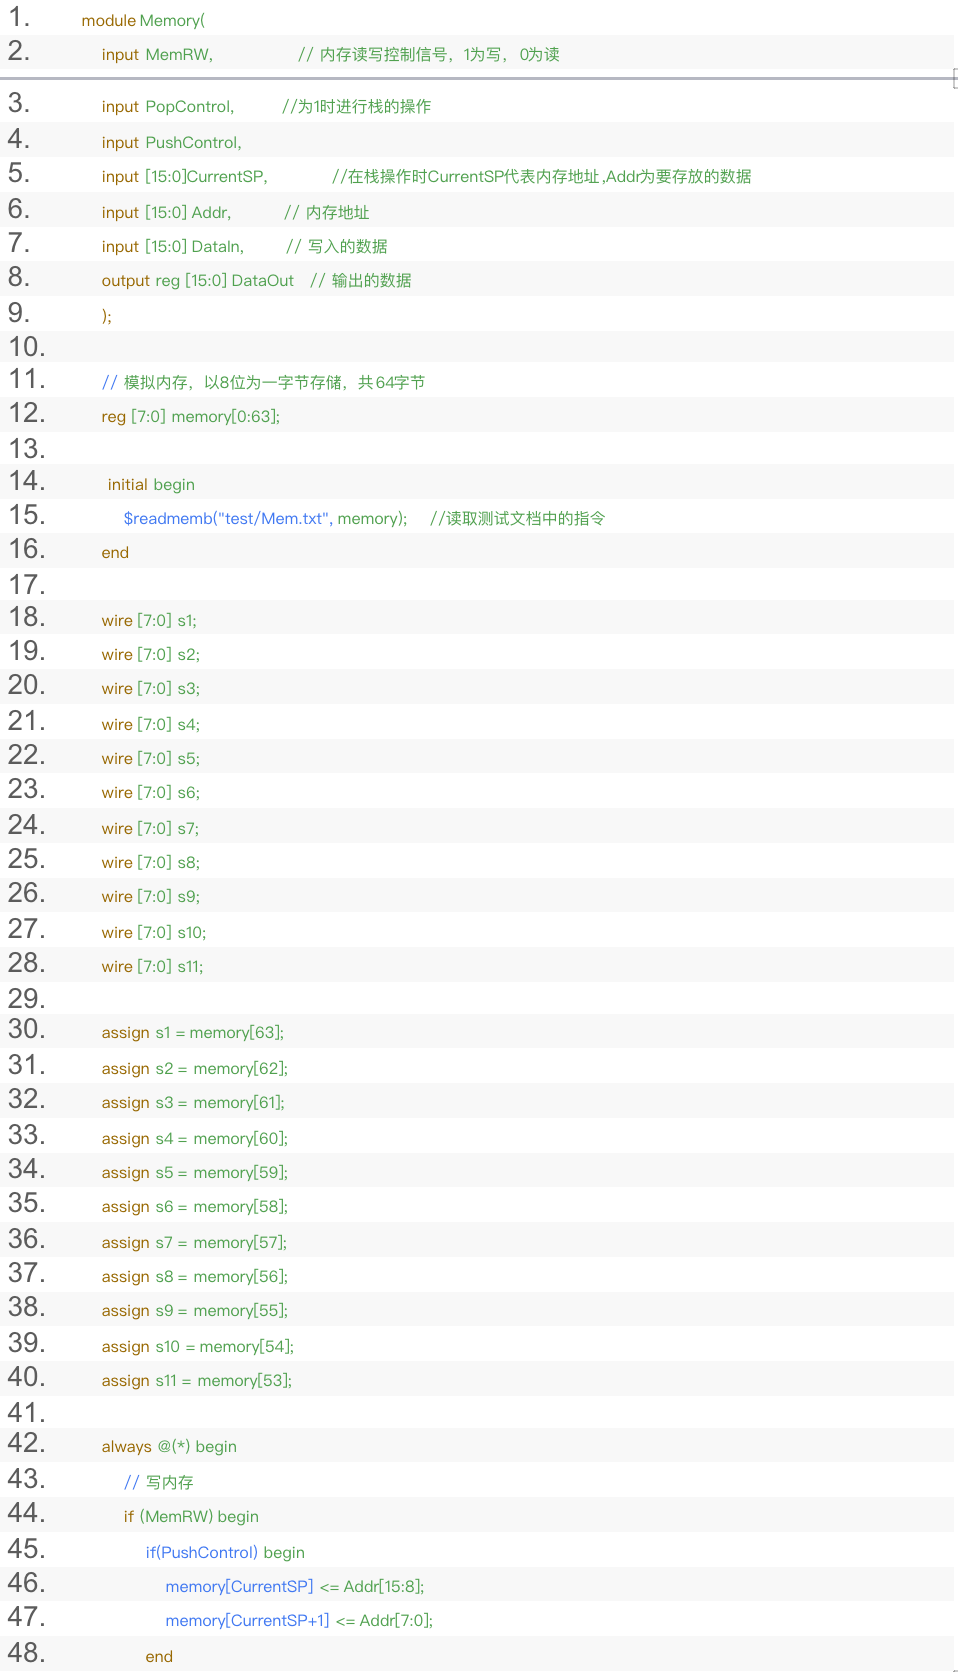
\includegraphics[width=0.8\textwidth]{pic/17.png}
  
    \end{figure}

\begin{figure}[H]
\centering
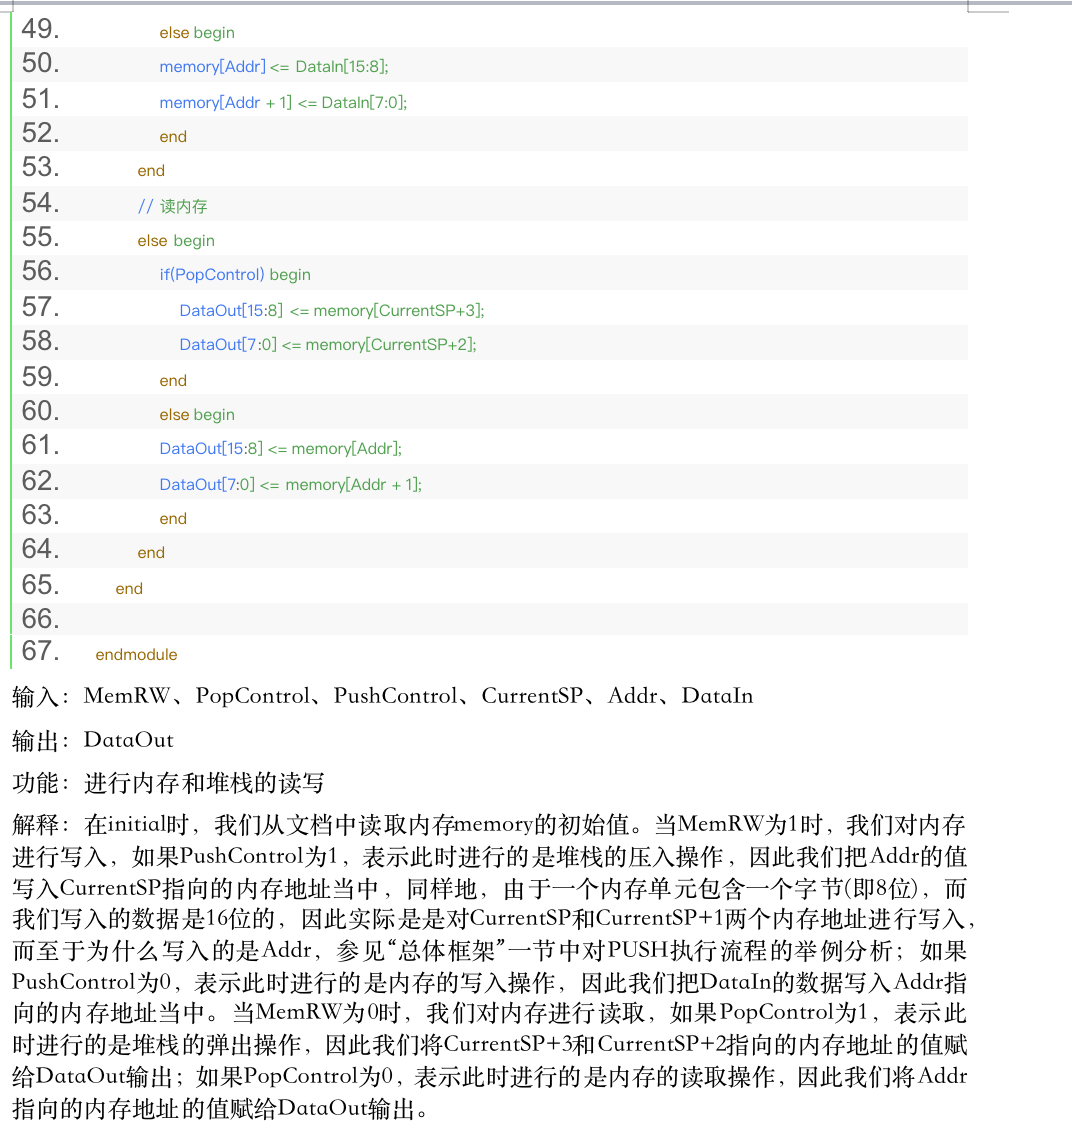
\includegraphics[width=0.8\textwidth]{pic/18.png}
\end{figure}

\subsection{module MUX}
\begin{figure}[H]
    \centering
    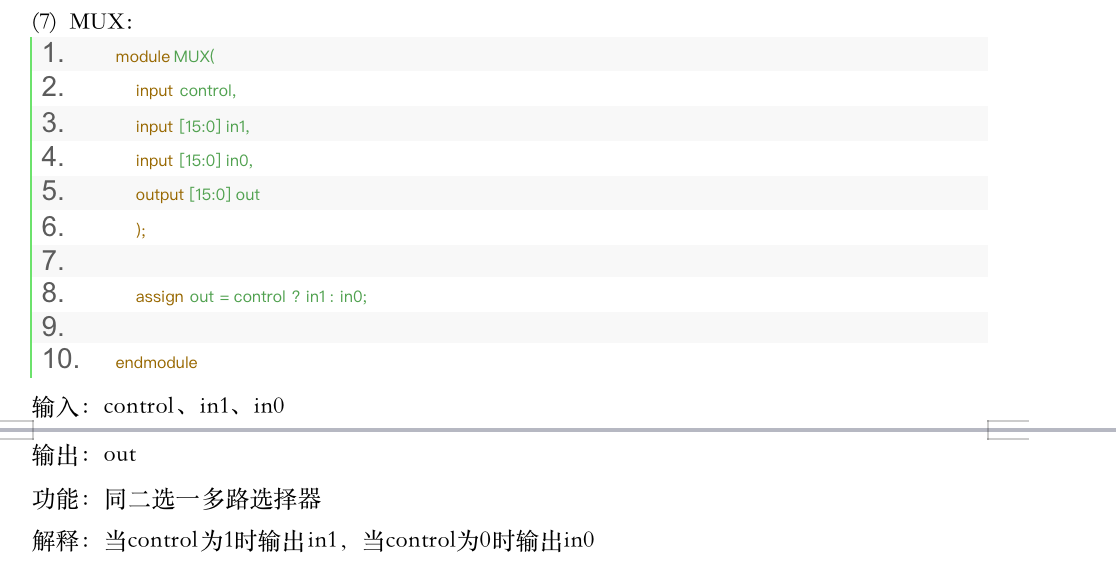
\includegraphics[width=0.8\textwidth]{pic/19.png}
    \end{figure}


\subsection{module SP}
\begin{figure}[H]
    \centering
    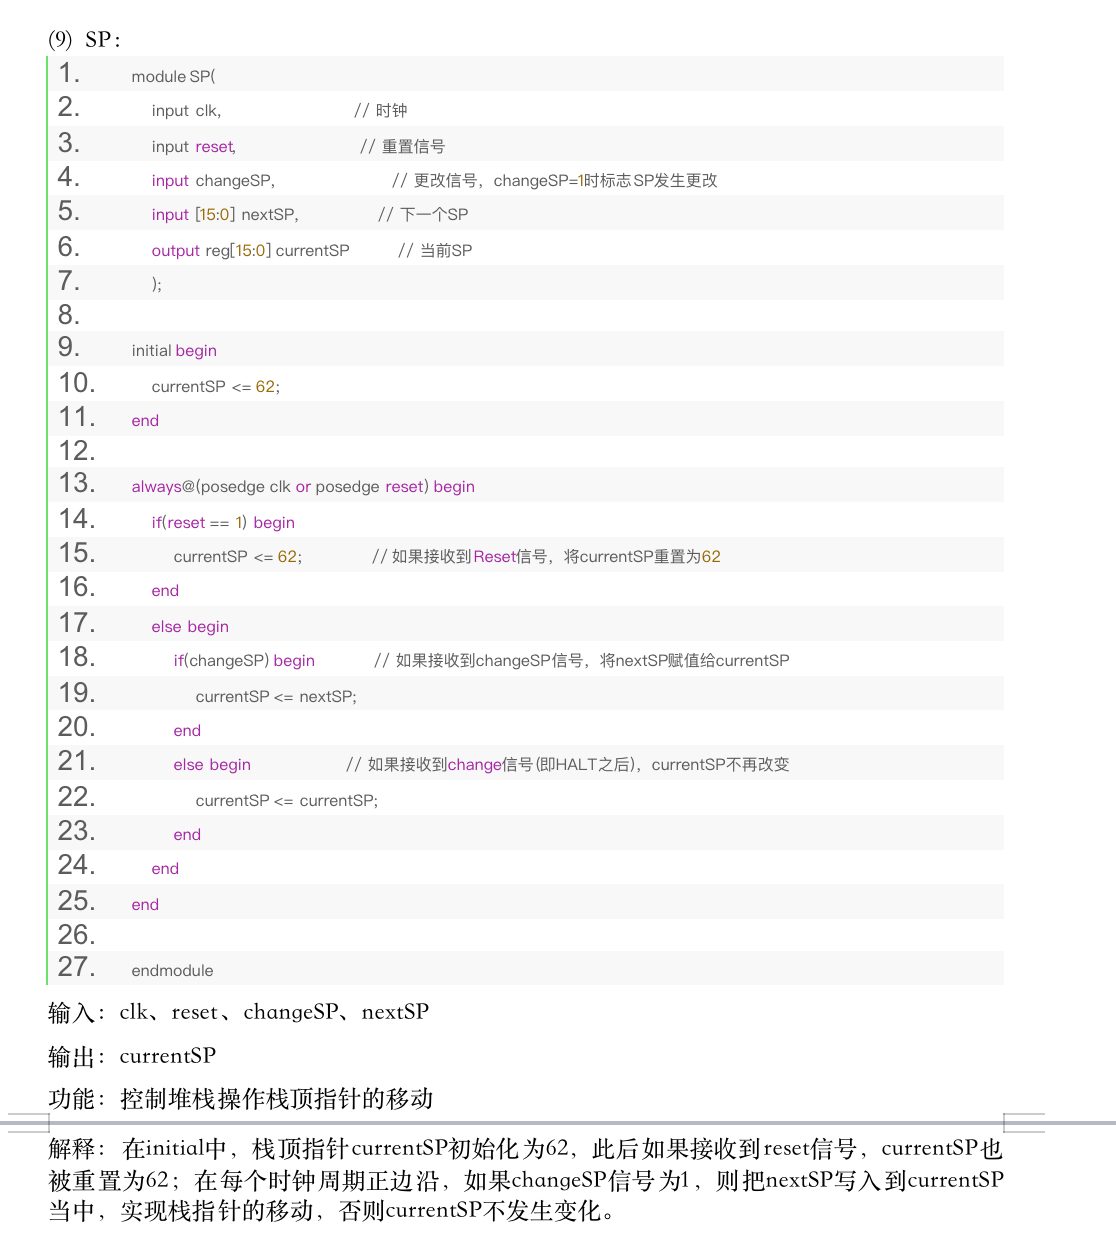
\includegraphics[width=1\textwidth]{pic/20.png}
    \end{figure}

\subsection{module SPMUX}
\begin{figure}[H]
    \centering
    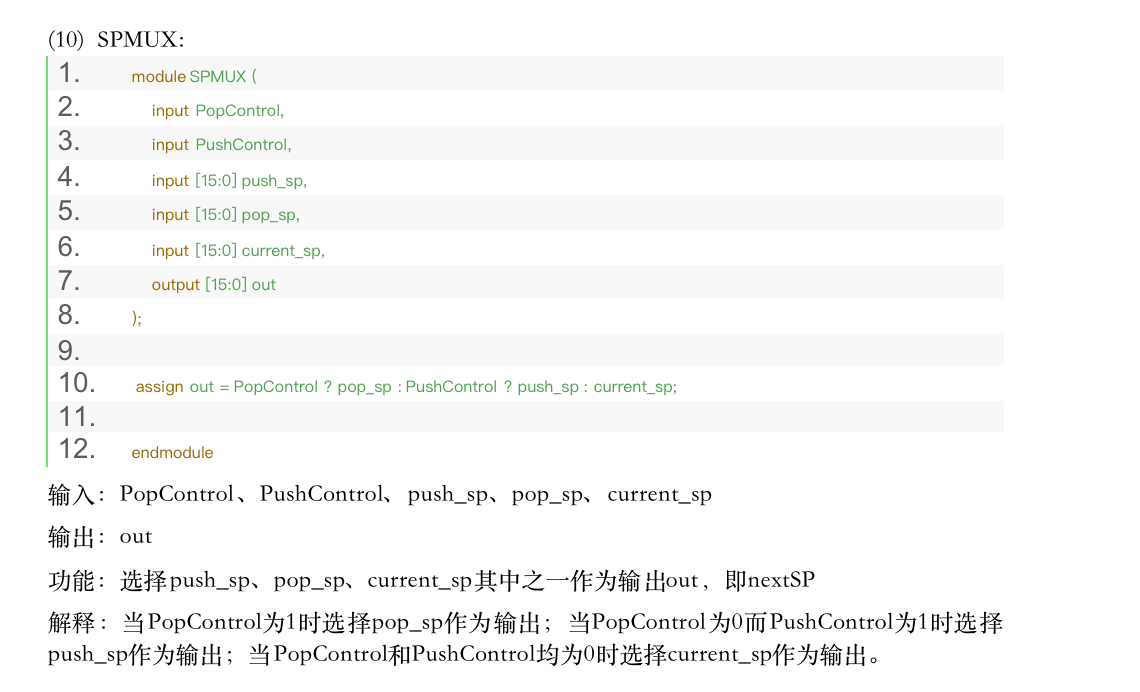
\includegraphics[width=0.8\textwidth]{pic/21.png}
    \end{figure}


\subsection{module ControlUnit}

这是整个CPU设计中最重要的部分,功能是根据输入的指令inst[15:0]和nzp,输出一系列控制信号,控制ALU和Memory等模块的工作,辅助指令的具体执行。由于这部分代码太长了,就不在这里给出了。对该模块的理解,其实就是对各控制信号的理解,控制信号的含义和功能可以参考“总体框架”中的控制信号表,而具体控制信号是如何控制其他模块的执行的可以参考“总体框架”中的数据通路图和对指令执行流程的解读,只要理解了以上这些内容,也就理解了ControlUnit的工作机制。

\subsection{module top}
顶层模块Top按照“总体框架”中的数据通路,将各模块连接起来,从而实现了单周期CPU的所有功能。


\section{测试方法}
我们的测试过程通过波形图仿真的方法来进行,由VScode+iverilog+gtkwave来进行的波形图仿真,
具体的方法参照了助教在语雀文档中提供的方法来进行:
\href{https://www.yuque.com/guahao-mjpno/bppkqw/ibdcd1}{yuque.com/guahao-mjpno} 

在具体的测试过程中:

\begin{figure}[H]
    \centering
    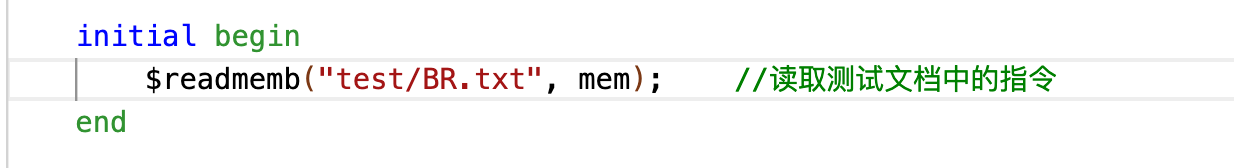
\includegraphics[width=0.5\textwidth]{pic/7.png}
    \caption{\label{pr}测试指令}
    \end{figure}
首先我们在test/文件夹下写好将要进行测试的机器码程序,在InstMem.v中对test/*.txt的测试文件进行读取,
然后编译运行全部的程序即可对整个设计进行验证.


\section{测试结果}

\subsection{验证ALU指令}

\begin{figure}[H]
    \centering
    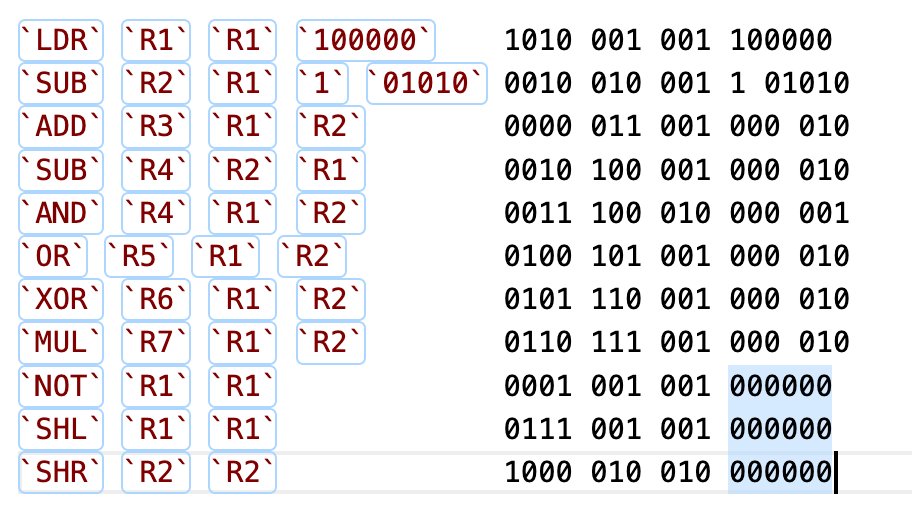
\includegraphics[width=0.5\textwidth]{pic/3.png}
    \caption{\label{pr}测试指令}
    \end{figure}
        
        
    
    
    
    \begin{figure}[H]
    \centering
    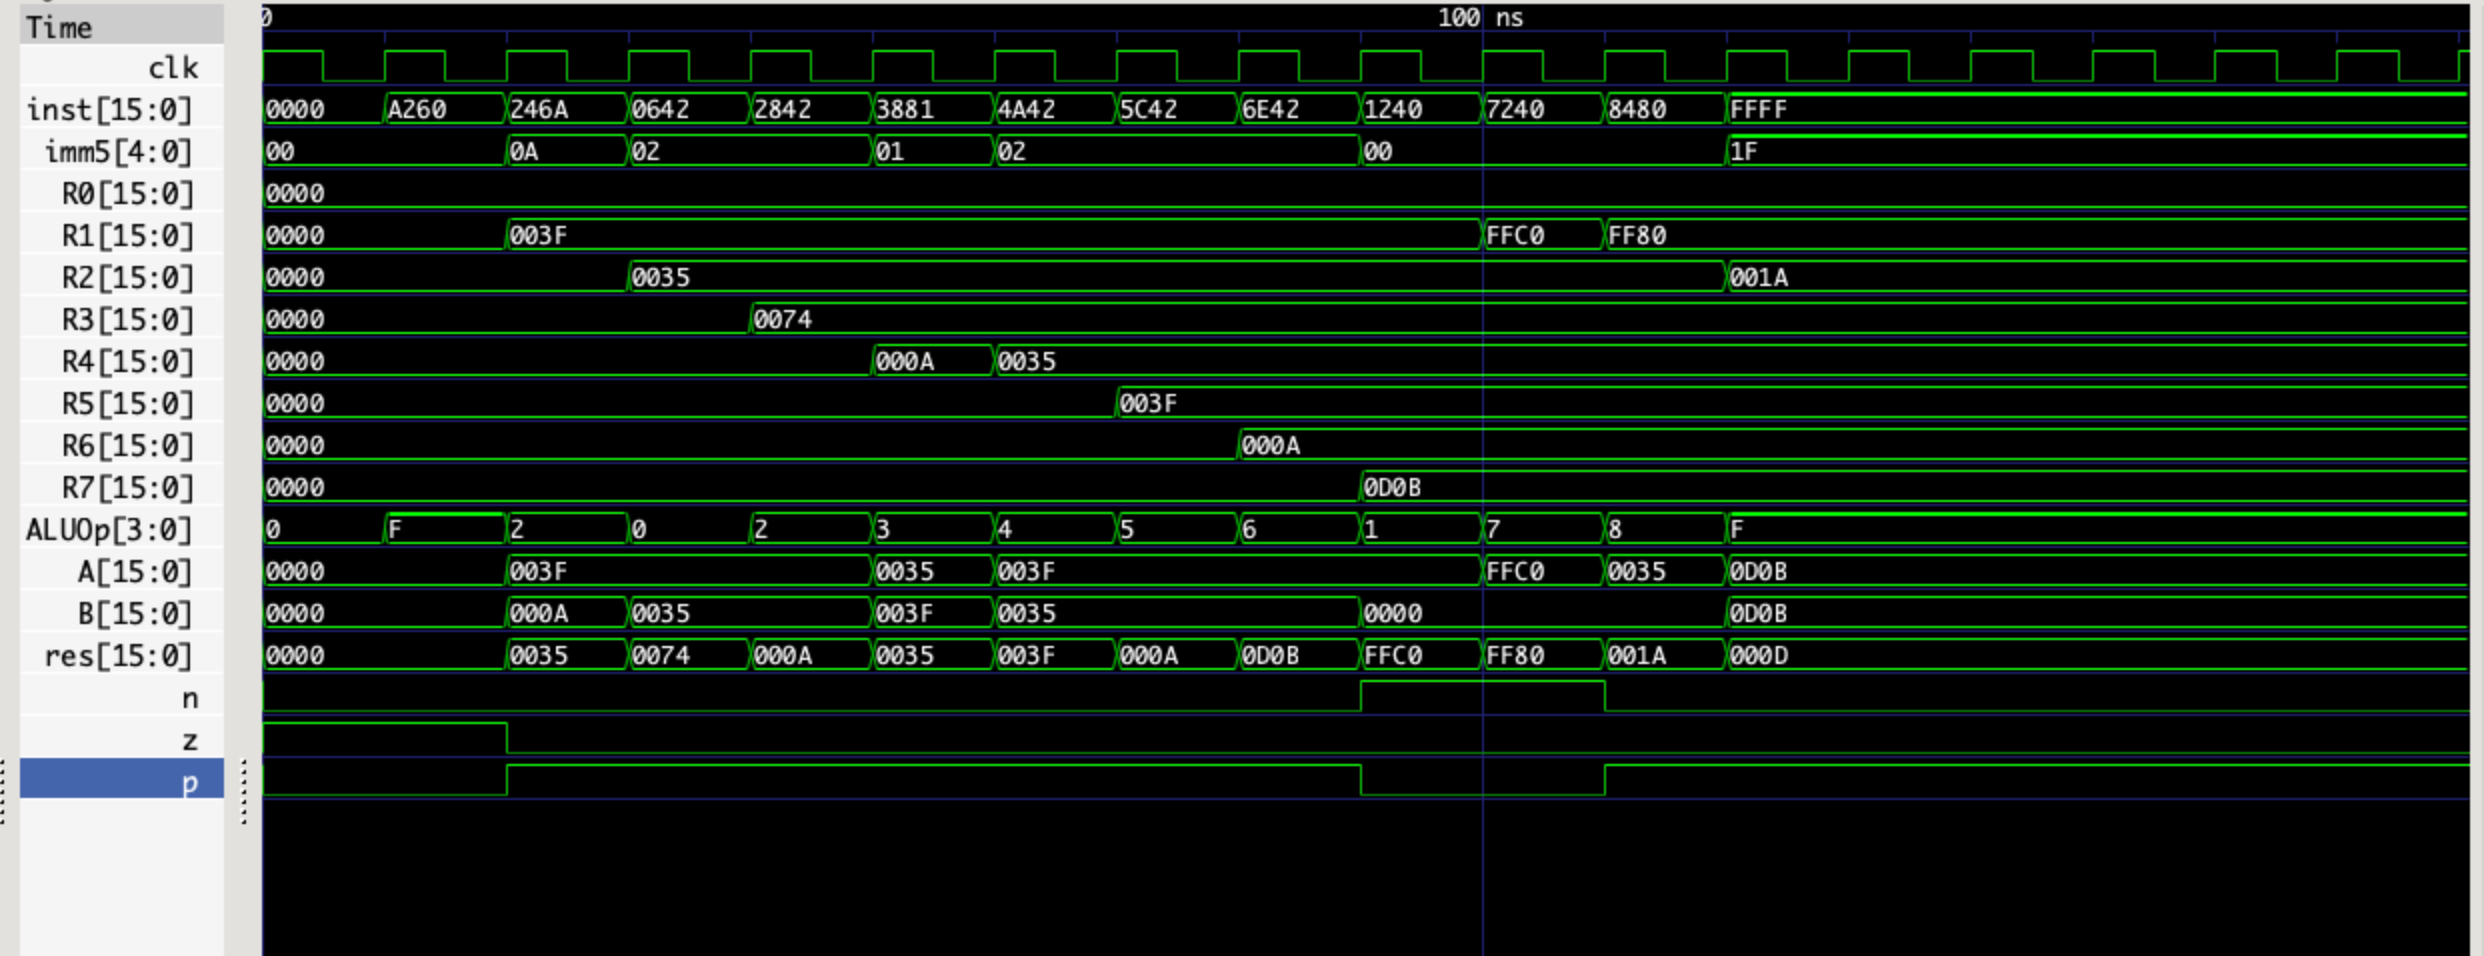
\includegraphics[width=1.2\textwidth]{pic/4.png}
    \caption{\label{pr}仿真结果}
    \end{figure}
    
这段测试代码进行了对ALU指令的验证和分析,在我们的设计中可以支持ADD,SUB,
AND,OR,XOR,MUL,NOT,SHL,SHR这些ALU指令的进行,从对应的测试波形我们可以
看到每次运算所对应的结果的正确获得,以及每次运算后n,z,p寄存器的正确变化,
对于其中的ALU指令我们同时支持了寄存器模式和立即数模式,在这两种模式下的ALU运算都可以正确进行.



\subsection{验证流程控制指令}

    
    



\begin{figure}[H]
\centering
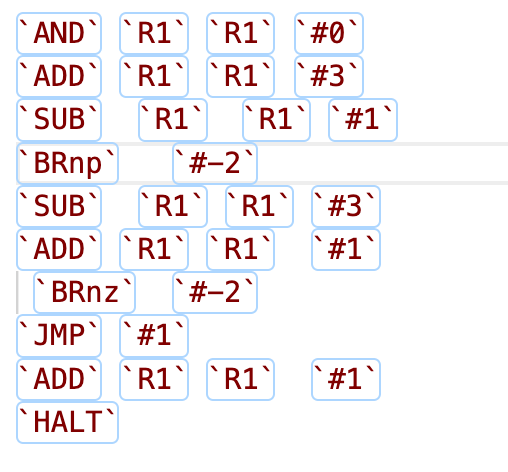
\includegraphics[width=0.5\textwidth]{pic/6.png}
\caption{\label{pr}仿真结果}
\end{figure}

\begin{figure}[H]
    \centering
    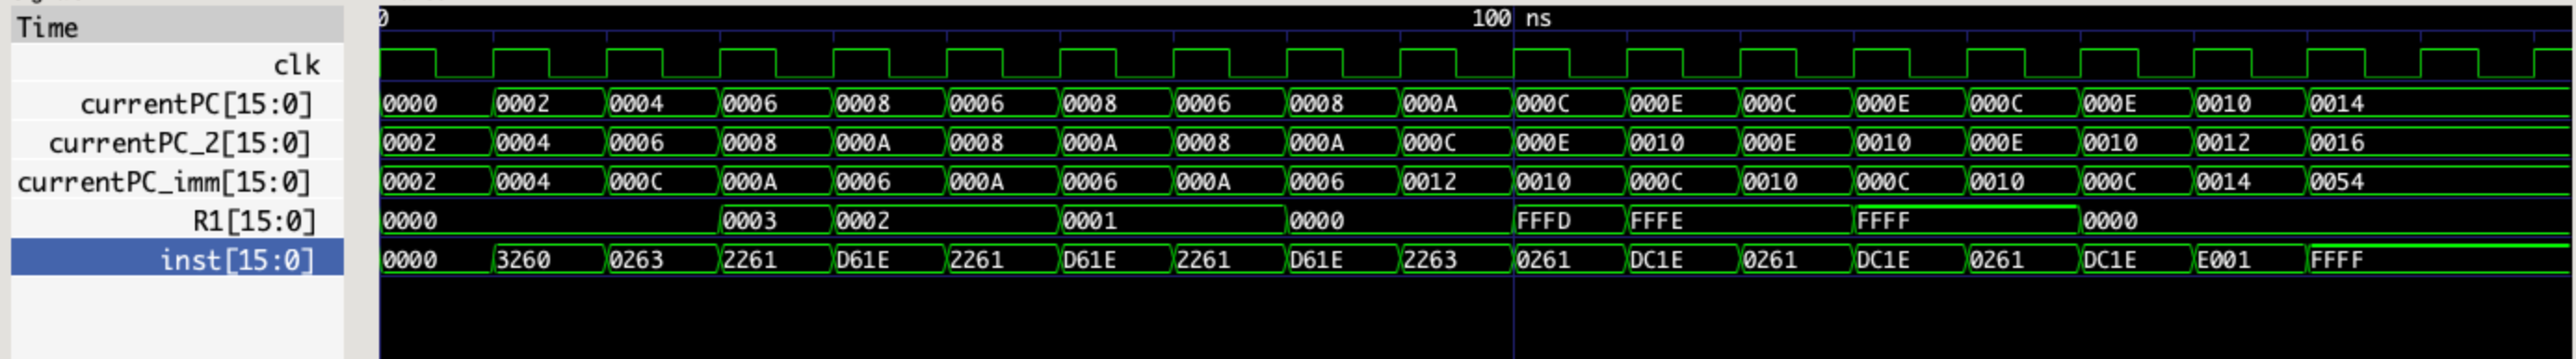
\includegraphics[width=1\textwidth]{pic/5.png}
    \caption{\label{pr}仿真结果}
    \end{figure}

BR指令(无条件跳转)和JMP指令(有条件跳转),是我们的设计中的流程控制相关的指令,
在这组测试程序中对流程控制指令进行了相应的测试,通过对currentPC的值的观察我们
可以看到BR所控制的循环过程的正确进行,以及最后一组JMP指令跳过了倒数第二步的ADD运算,
在波形图中也得到了正确的结果.



\subsection{验证指令:PUSH、POP}

\begin{figure}[H]
\centering
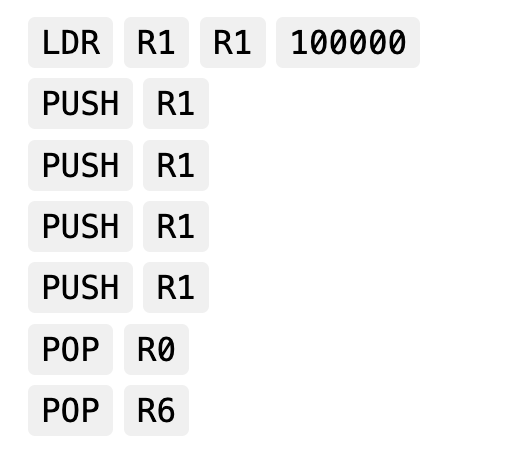
\includegraphics[width=0.3\textwidth]{pic/2.png}
\caption{\label{pr}测试指令}
\end{figure}
    
\begin{figure}[H]
    \centering
    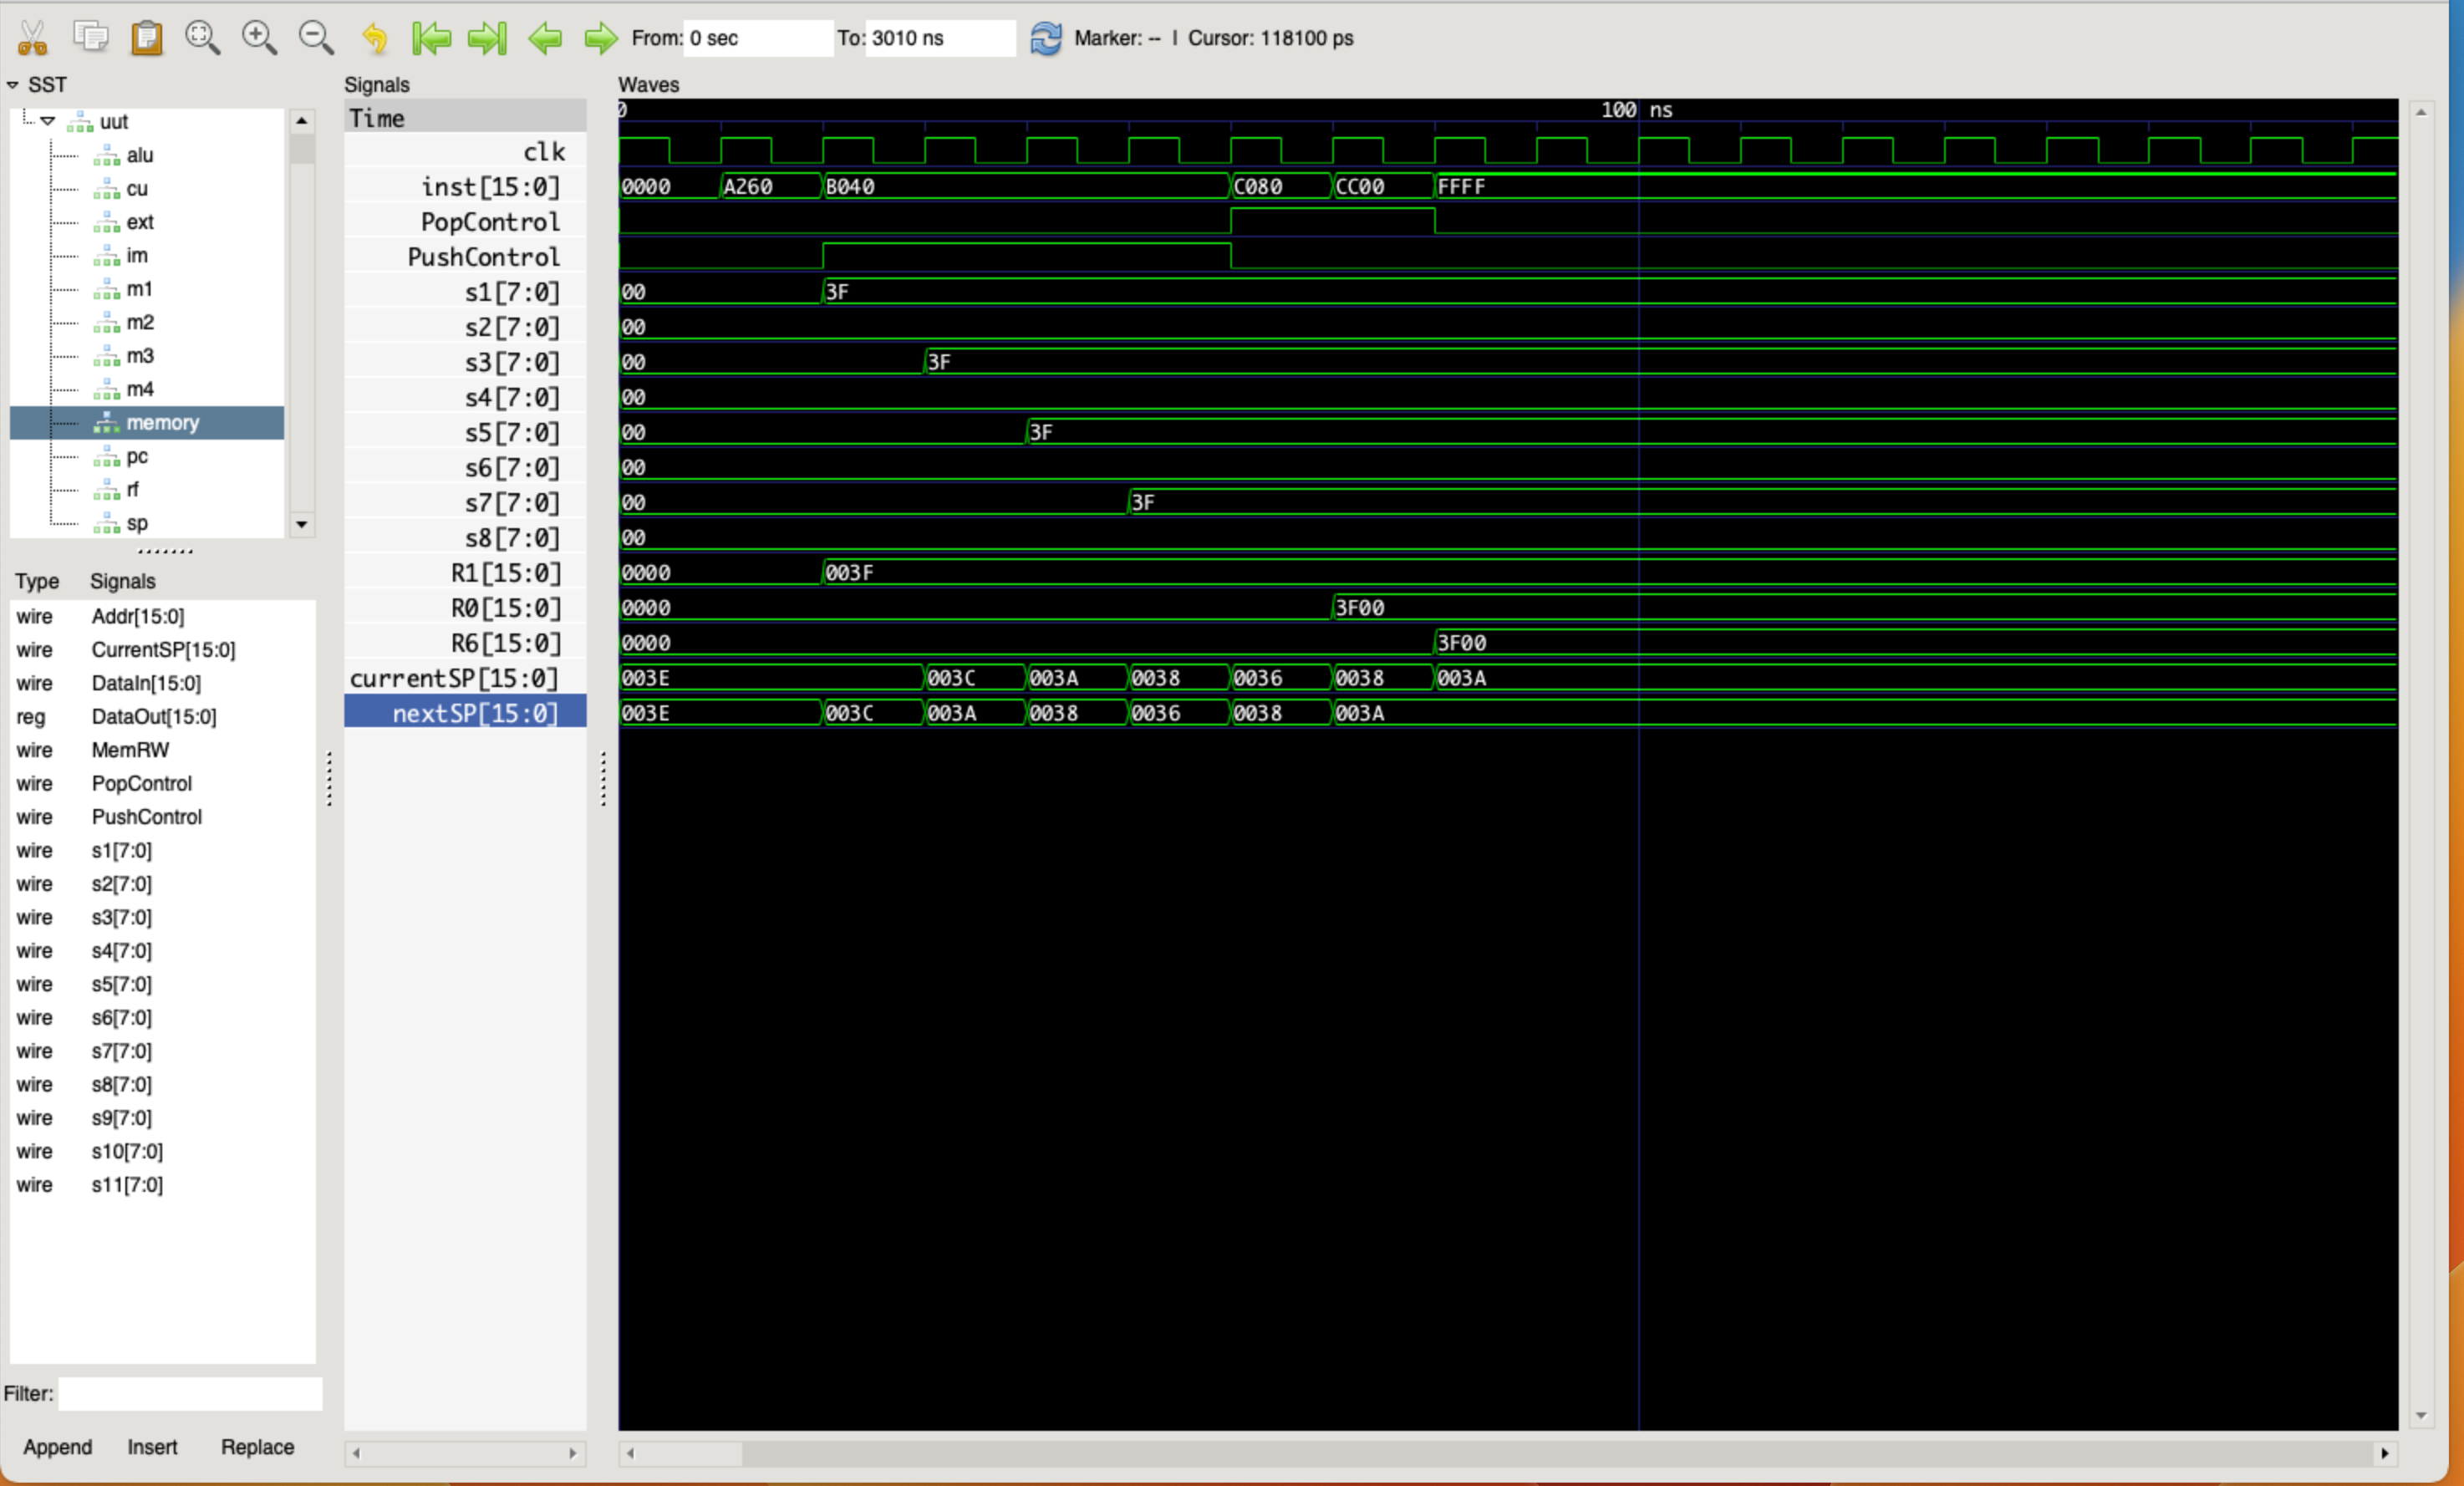
\includegraphics[width=1.2\textwidth]{pic/1.png}
    \caption{\label{pr}仿真结果}
    \end{figure}
    









这一组测试用于对push和pop的这一对指令的验证和分析,首先通过LDR指令让R1获得
在Mem.txt文件中存储的数据,然后进行了三次PUSH指令和两次POP指令,在波形图中我们
可以看到PushControl和PopControl的信号在PUSH和POP时可以进行正确的响应,
通过currentSP我们可以看到栈指针的正确移动,在PUSH时栈指针向上移动其值减2,在POP
时栈指针向下移动其值加2.

在测试时我们设置了s1~s8的wire类型变量用于显示观察Mem的内存情况,可以看到在PUSH过程中内存的正确变化.
在POP时观察输出到的对应寄存器我们可以看到R0,R6获得了栈中数值的逆序结果.

\subsection{运行计算斐波那契数指令}
设计如下的指令来在寄存器中展示斐波那契数列
\begin{figure}[H]
    \centering
    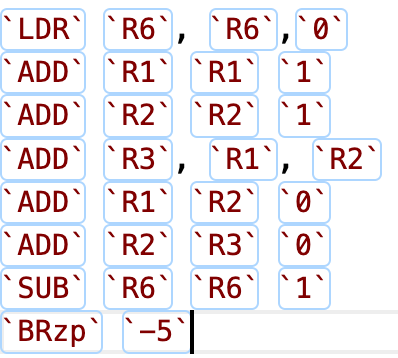
\includegraphics[width=0.5\textwidth]{1.png}
   
    \end{figure}

测试的波形结果如下:
\begin{figure}[H]
    \centering
    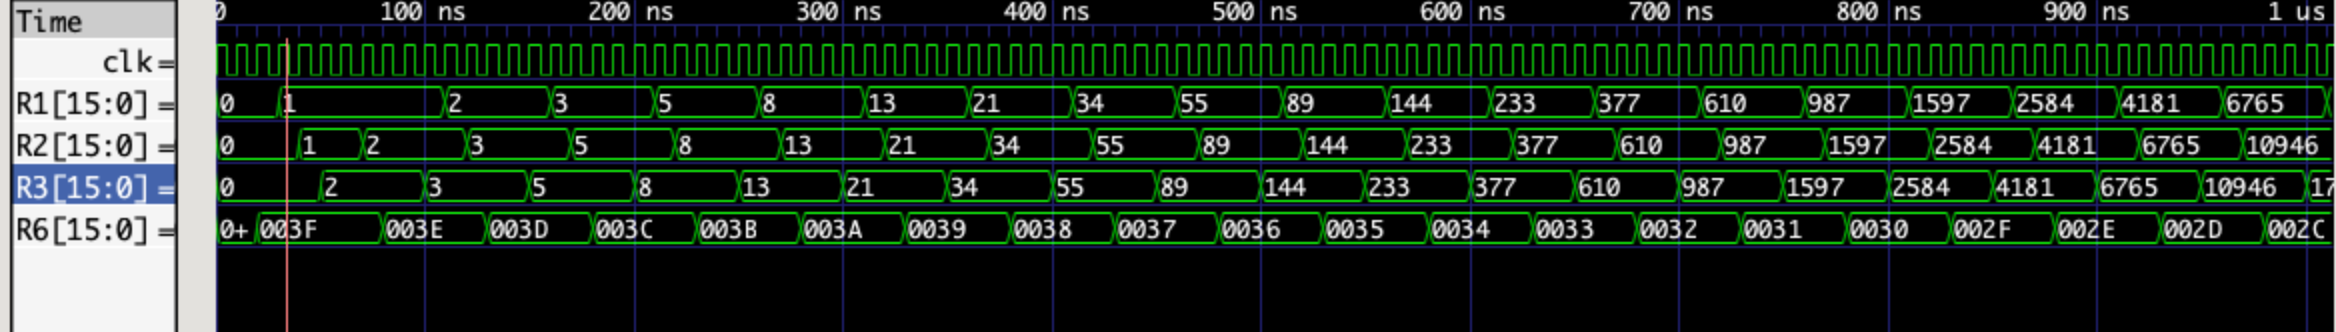
\includegraphics[width=1\textwidth]{2.png}
   
    \end{figure}

R6是循环的计数器,观察寄存器R1,R2,R3可以看到斐波那契数的结果,这一组指令主要验证了
ALU运算的指令和流程控制指令BR,同时验证了所设计的指令集可以完成对简单应用代码的正确处理.


\section{成员贡献度}
雷远航:50$\%$

祝广程:50$\%$


\section{附录:github commit 记录}
commit的内容以一下超链接形式给出,点击即可查看:

\href{https://github.com/lyh031026huahuo1234/FPGA/commit/c23338e3e2d618f0f60e147ae3171259653f18c0}{-final project-} 

\href{https://github.com/lyh031026huahuo1234/FPGA/commit/5dc46de748a9b6c0a2f98d666d9cafa90616ae1c}{-merge version3's RegFile.v to version4-} 

\href{https://github.com/lyh031026huahuo1234/FPGA/commit/8ab835e84b8704036dd17177fd21a39e7fc7dbb3}{-add push and pop,change BR-}

\href{https://github.com/lyh031026huahuo1234/FPGA/commit/6f65d11591ff371db7cb10cd4e8afc1c09ef3051}{-debug and test-}


\href{https://github.com/lyh031026huahuo1234/FPGA/commit/05c2abe0720445d591cb86a88e2cd1ae73d90c9c}{-modules for new organization-}

\href{https://github.com/lyh031026huahuo1234/FPGA/commit/75b1552252936fcbecede27b80b03d2d783391ce}{-debug-}

\href{https://github.com/lyh031026huahuo1234/FPGA/commit/ee0a76e611e4321e34963ad228e82693b8a2db38}{-commit some syntax error-}

\href{https://github.com/lyh031026huahuo1234/FPGA/commit/121aa80b3b038370c69262b26d2ba4924143cab1}{-Some module corrections and improvements-}

\href{https://github.com/lyh031026huahuo1234/FPGA/commit/7aa8c0ca0500cd12a02199083dd7ad8dca750284}{-commit top module design-}

\href{https://github.com/lyh031026huahuo1234/FPGA/commit/035580ca64eb6be3e56a62e0d6f96c69ec52480c}{-Module reorganization and design-}

\href{https://github.com/lyh031026huahuo1234/FPGA/commit/b7df2657a48e5a9d9b2984d78ff0564daa588588}{-commit MUL module-}

\href{https://github.com/lyh031026huahuo1234/FPGA/commit/6cd80229a412af0df88642db99a90405ca530a39}{-main-}

\section{附录:ISA}
\subsection{ALU指令}

\begin{figure}[H]
    \centering
    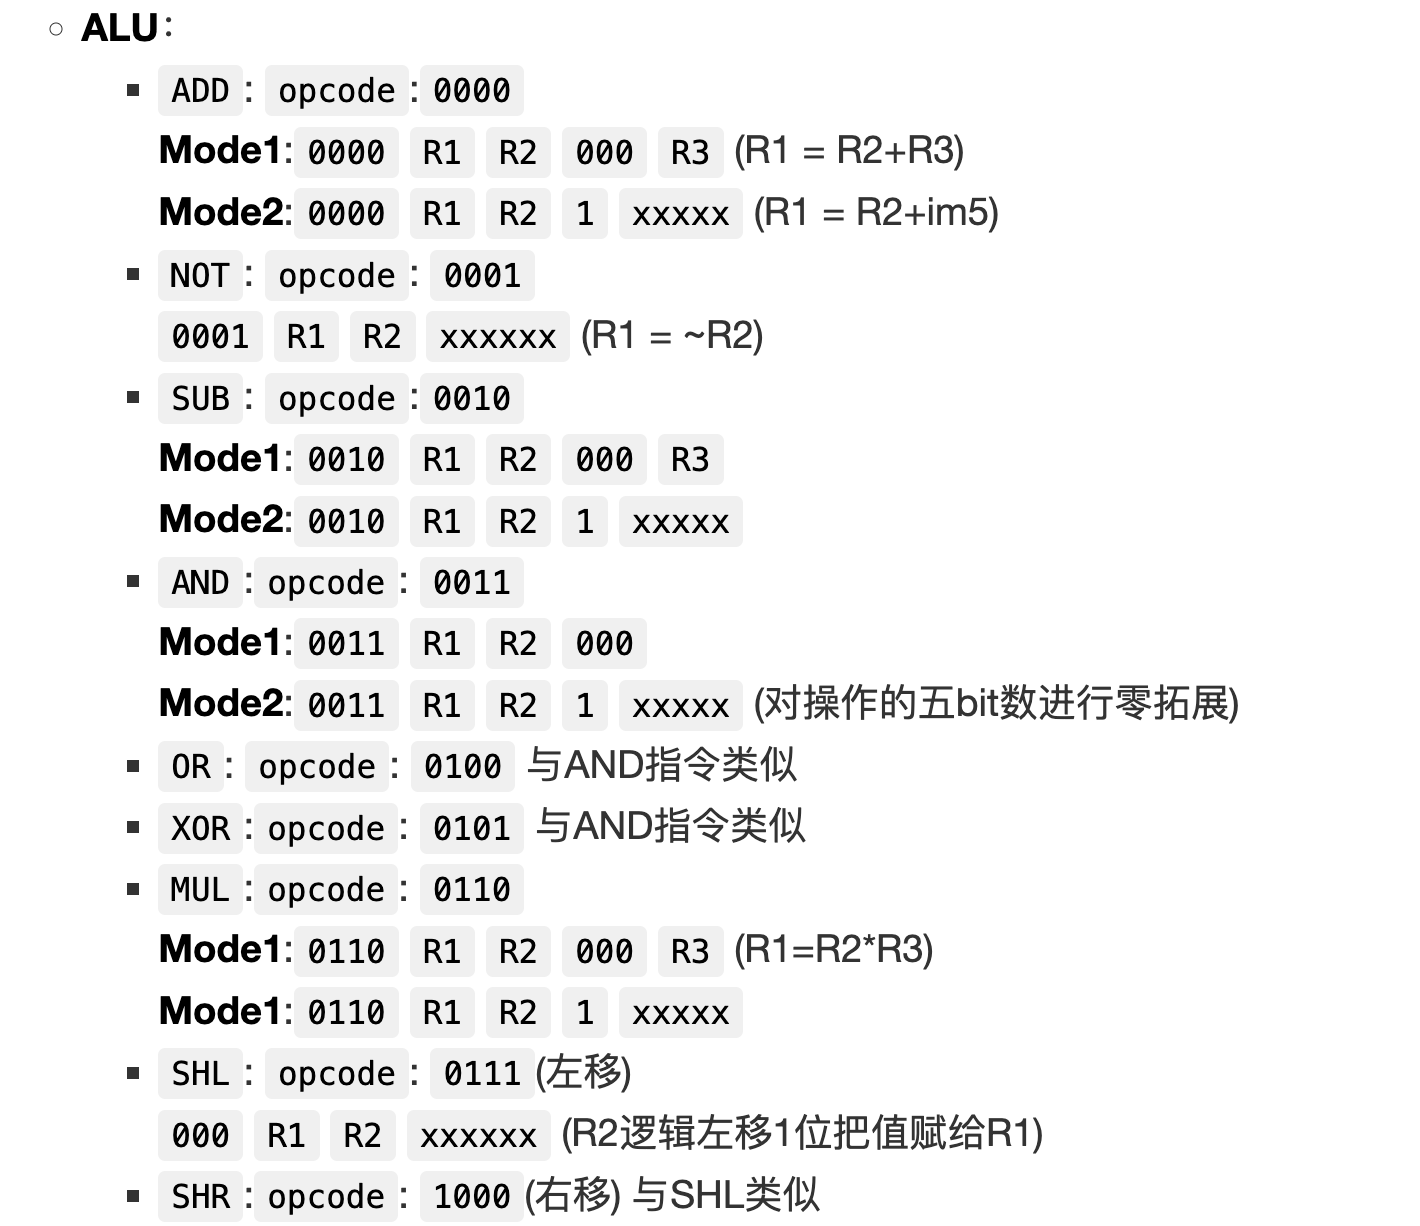
\includegraphics[width=1\textwidth]{pic/22.png}
   
    \end{figure}
    

\subsection{存储指令}
\begin{figure}[H]
    \centering
    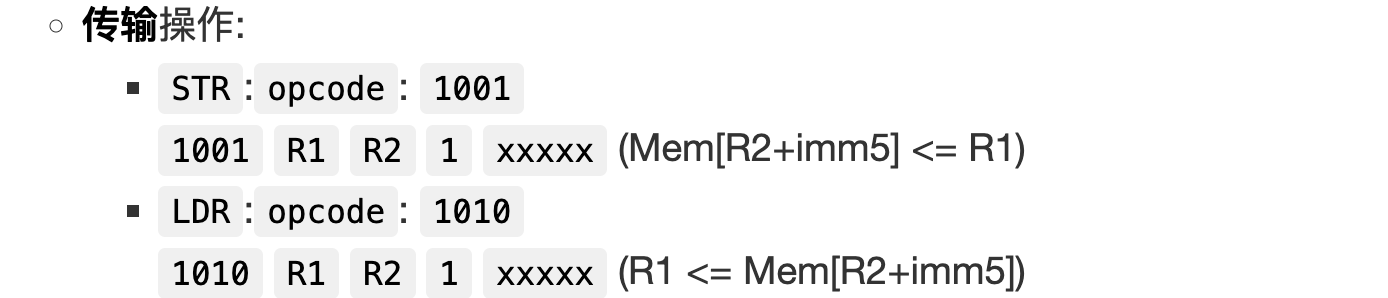
\includegraphics[width=1\textwidth]{pic/23.png}
   
    \end{figure}

\subsection{流程控制指令}
\begin{figure}[H]
    \centering
    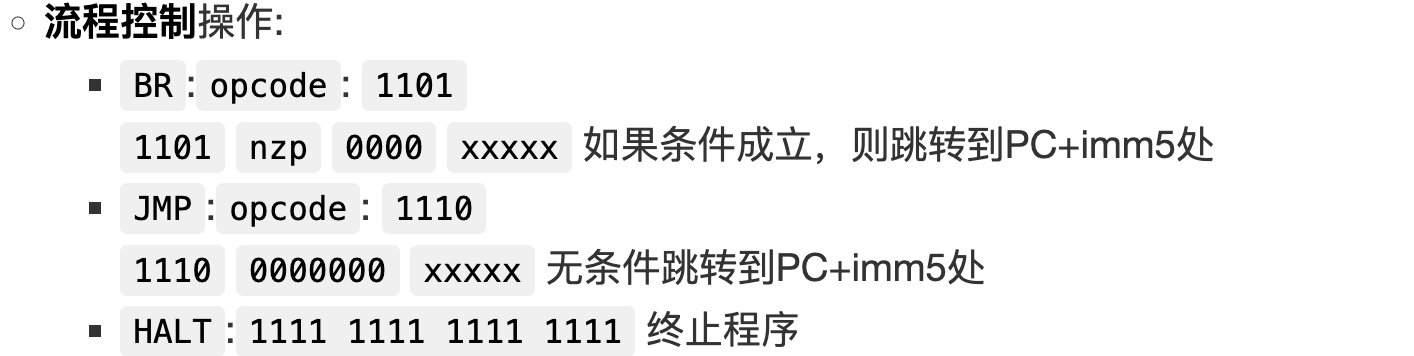
\includegraphics[width=1\textwidth]{pic/24.png}
   
    \end{figure}

\subsection{堆栈操作指令}
\begin{figure}[H]
    \centering
    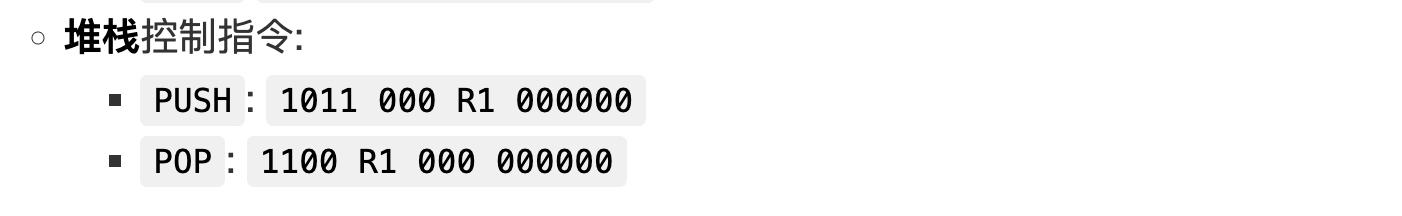
\includegraphics[width=1\textwidth]{pic/25.png}
   
    \end{figure}




\end{document}